\PassOptionsToPackage{unicode=true}{hyperref} % options for packages loaded elsewhere
\PassOptionsToPackage{hyphens}{url}
%
\documentclass[
]{article}
\usepackage{lmodern}
\usepackage{amssymb,amsmath}
\usepackage{ifxetex,ifluatex}
\ifnum 0\ifxetex 1\fi\ifluatex 1\fi=0 % if pdftex
  \usepackage[T1]{fontenc}
  \usepackage[utf8]{inputenc}
  \usepackage{textcomp} % provides euro and other symbols
\else % if luatex or xelatex
  \usepackage{unicode-math}
  \defaultfontfeatures{Scale=MatchLowercase}
  \defaultfontfeatures[\rmfamily]{Ligatures=TeX,Scale=1}
\fi
% use upquote if available, for straight quotes in verbatim environments
\IfFileExists{upquote.sty}{\usepackage{upquote}}{}
\IfFileExists{microtype.sty}{% use microtype if available
  \usepackage[]{microtype}
  \UseMicrotypeSet[protrusion]{basicmath} % disable protrusion for tt fonts
}{}
\makeatletter
\@ifundefined{KOMAClassName}{% if non-KOMA class
  \IfFileExists{parskip.sty}{%
    \usepackage{parskip}
  }{% else
    \setlength{\parindent}{0pt}
    \setlength{\parskip}{6pt plus 2pt minus 1pt}}
}{% if KOMA class
  \KOMAoptions{parskip=half}}
\makeatother
\usepackage{xcolor}
\IfFileExists{xurl.sty}{\usepackage{xurl}}{} % add URL line breaks if available
\IfFileExists{bookmark.sty}{\usepackage{bookmark}}{\usepackage{hyperref}}
\hypersetup{
  pdftitle={Generalized Linear Mixed/Multilevel Models (GLMMs)},
  pdfauthor={T. Florian Jaeger},
  pdfborder={0 0 0},
  breaklinks=true}
\urlstyle{same}  % don't use monospace font for urls
\usepackage[margin=2cm]{geometry}
\usepackage{color}
\usepackage{fancyvrb}
\newcommand{\VerbBar}{|}
\newcommand{\VERB}{\Verb[commandchars=\\\{\}]}
\DefineVerbatimEnvironment{Highlighting}{Verbatim}{commandchars=\\\{\}}
% Add ',fontsize=\small' for more characters per line
\usepackage{framed}
\definecolor{shadecolor}{RGB}{248,248,248}
\newenvironment{Shaded}{\begin{snugshade}}{\end{snugshade}}
\newcommand{\AlertTok}[1]{\textcolor[rgb]{0.94,0.16,0.16}{#1}}
\newcommand{\AnnotationTok}[1]{\textcolor[rgb]{0.56,0.35,0.01}{\textbf{\textit{#1}}}}
\newcommand{\AttributeTok}[1]{\textcolor[rgb]{0.77,0.63,0.00}{#1}}
\newcommand{\BaseNTok}[1]{\textcolor[rgb]{0.00,0.00,0.81}{#1}}
\newcommand{\BuiltInTok}[1]{#1}
\newcommand{\CharTok}[1]{\textcolor[rgb]{0.31,0.60,0.02}{#1}}
\newcommand{\CommentTok}[1]{\textcolor[rgb]{0.56,0.35,0.01}{\textit{#1}}}
\newcommand{\CommentVarTok}[1]{\textcolor[rgb]{0.56,0.35,0.01}{\textbf{\textit{#1}}}}
\newcommand{\ConstantTok}[1]{\textcolor[rgb]{0.00,0.00,0.00}{#1}}
\newcommand{\ControlFlowTok}[1]{\textcolor[rgb]{0.13,0.29,0.53}{\textbf{#1}}}
\newcommand{\DataTypeTok}[1]{\textcolor[rgb]{0.13,0.29,0.53}{#1}}
\newcommand{\DecValTok}[1]{\textcolor[rgb]{0.00,0.00,0.81}{#1}}
\newcommand{\DocumentationTok}[1]{\textcolor[rgb]{0.56,0.35,0.01}{\textbf{\textit{#1}}}}
\newcommand{\ErrorTok}[1]{\textcolor[rgb]{0.64,0.00,0.00}{\textbf{#1}}}
\newcommand{\ExtensionTok}[1]{#1}
\newcommand{\FloatTok}[1]{\textcolor[rgb]{0.00,0.00,0.81}{#1}}
\newcommand{\FunctionTok}[1]{\textcolor[rgb]{0.00,0.00,0.00}{#1}}
\newcommand{\ImportTok}[1]{#1}
\newcommand{\InformationTok}[1]{\textcolor[rgb]{0.56,0.35,0.01}{\textbf{\textit{#1}}}}
\newcommand{\KeywordTok}[1]{\textcolor[rgb]{0.13,0.29,0.53}{\textbf{#1}}}
\newcommand{\NormalTok}[1]{#1}
\newcommand{\OperatorTok}[1]{\textcolor[rgb]{0.81,0.36,0.00}{\textbf{#1}}}
\newcommand{\OtherTok}[1]{\textcolor[rgb]{0.56,0.35,0.01}{#1}}
\newcommand{\PreprocessorTok}[1]{\textcolor[rgb]{0.56,0.35,0.01}{\textit{#1}}}
\newcommand{\RegionMarkerTok}[1]{#1}
\newcommand{\SpecialCharTok}[1]{\textcolor[rgb]{0.00,0.00,0.00}{#1}}
\newcommand{\SpecialStringTok}[1]{\textcolor[rgb]{0.31,0.60,0.02}{#1}}
\newcommand{\StringTok}[1]{\textcolor[rgb]{0.31,0.60,0.02}{#1}}
\newcommand{\VariableTok}[1]{\textcolor[rgb]{0.00,0.00,0.00}{#1}}
\newcommand{\VerbatimStringTok}[1]{\textcolor[rgb]{0.31,0.60,0.02}{#1}}
\newcommand{\WarningTok}[1]{\textcolor[rgb]{0.56,0.35,0.01}{\textbf{\textit{#1}}}}
\usepackage{graphicx,grffile}
\makeatletter
\def\maxwidth{\ifdim\Gin@nat@width>\linewidth\linewidth\else\Gin@nat@width\fi}
\def\maxheight{\ifdim\Gin@nat@height>\textheight\textheight\else\Gin@nat@height\fi}
\makeatother
% Scale images if necessary, so that they will not overflow the page
% margins by default, and it is still possible to overwrite the defaults
% using explicit options in \includegraphics[width, height, ...]{}
\setkeys{Gin}{width=\maxwidth,height=\maxheight,keepaspectratio}
\setlength{\emergencystretch}{3em}  % prevent overfull lines
\providecommand{\tightlist}{%
  \setlength{\itemsep}{0pt}\setlength{\parskip}{0pt}}
\setcounter{secnumdepth}{5}
% Redefines (sub)paragraphs to behave more like sections
\ifx\paragraph\undefined\else
  \let\oldparagraph\paragraph
  \renewcommand{\paragraph}[1]{\oldparagraph{#1}\mbox{}}
\fi
\ifx\subparagraph\undefined\else
  \let\oldsubparagraph\subparagraph
  \renewcommand{\subparagraph}[1]{\oldsubparagraph{#1}\mbox{}}
\fi

% set default figure placement to htbp
\makeatletter
\def\fps@figure{htbp}
\makeatother

\usepackage{booktabs}
\usepackage{siunitx}
\usepackage{tabto}
\usepackage{soul}
\usepackage{xcolor}
\usepackage{placeins}
\usepackage{lscape}
\newcommand{\blandscape}{\begin{landscape}}
\newcommand{\elandscape}{\end{landscape}}
\makeatletter\renewcommand{\fps@table}{!ht}\makeatother
\setstcolor{red}
\usepackage{sectsty}
\sectionfont{\color{blue}}
\subsectionfont{\color{blue}}
\subsubsectionfont{\color{darkgray}}
\usepackage{caption}
\usepackage{subcaption}
\usepackage{tikz}
\usepackage{url}
\usetikzlibrary{bayesnet}

\title{Generalized Linear Mixed/Multilevel Models (GLMMs)}
\usepackage{etoolbox}
\makeatletter
\providecommand{\subtitle}[1]{% add subtitle to \maketitle
  \apptocmd{\@title}{\par {\large #1 \par}}{}{}
}
\makeatother
\subtitle{An applied tutorial}
\author{T. Florian Jaeger}
\date{\today}

\begin{document}
\maketitle

{
\setcounter{tocdepth}{4}
\tableofcontents
}
\hypertarget{to-do}{%
\section{TO DO}\label{to-do}}

get trial level data

make visualization read up on weibull

\begin{figure}
  \centering
  \begin{subfigure}[b]{0.45\textwidth}
  \tikz{ %
    \node[obs] (outcome) {$y_i$} ; %
    \factor[above=of outcome] {distribution} {left: \textcolor{orange}{distribution $f$}} {} {}; %
    \node[det, above=of distribution] (mu) {$\mu_i$} ; %
    \factor[above=of mu] {link} {left: \textcolor{blue}{inverse link $g^{-1}$}} {} {}; %
    \node[obs, above=of link] (X) {$x_i$} ; %
    \node[latent, right=of X] (beta) {$\beta$} ; %
    % plates
    \plate[inner sep=0.12cm, xshift=-0.06cm, yshift=0.06cm] {plate1} {(mu) (distribution) (link) (X) (outcome)} {$\forall i=1 \ldots N $}; %
    \edge {distribution} {outcome} ; %
    \edge {mu} {distribution} ; %
    \edge {link} {mu} ; %
    \edge {X, beta} {link} ; %
  }
  \caption{Generalized linear model (GLM)}
  \end{subfigure}
  \hfill
  \begin{subfigure}[b]{0.45\textwidth}
  \tikz{ %
    \node[obs] (outcome) {$y_{i,j}$} ; %
    \factor[above=of outcome] {distribution} {left: \textcolor{orange}{$f$}} {} {}; %
    \node[det, above=of distribution] (mu) {$\mu_{i,j}$} ; %
    \factor[above=of mu] {link} {left: \textcolor{blue}{$g^{-1}$}} {} {}; %
    \node[obs, above=of link] (X) {$x_{i,j}$} ; %
    \node[latent, right=of link] (betas) {$\beta_j$} ; %
    \factor[right=of betas] {group} {below:$\mathcal{N}$} {} {}; %
    \node[latent, above=of group] (Sigma) {$\Sigma$} ; %
    \node[latent, right=of group] (beta) {$\beta$} ; %
    \node[obs, right=of X, above=of betas] (grouplevel) {$z_j$} ; %
    % plates
    \plate[inner sep=0.12cm, xshift=-0.06cm, yshift=0.06cm] {plate1} {(mu) (distribution) (link) (X) (outcome)} {$N $}; %
    \plate[inner sep=0.12cm, xshift=-0.06cm, yshift=0.06cm] {plate2} {(mu) (distribution) (link) (betas) (X) (outcome) (grouplevel) (plate1) } {$M $}; %
    \edge {distribution} {outcome} ; %
    \edge {mu} {distribution} ; %
    \edge {link} {mu} ; %
    \edge {X, betas, grouplevel} {link} ; %
    \edge {group} {betas} ; %
    \edge {Sigma, beta} {group} ; %
  }
  \caption{Generalized linear mixed model (GLMM)}
  \end{subfigure}
  \caption{The three components of the GLM: the linear predictor ($X\beta$), the link function $g$, and the distribution $f$. For the GLMM, $z_j$ is the $j$th level of the grouping variable $z$, which select which $\beta_j$ is to be chosen for the present case.}
\end{figure}

\begin{figure}
  \centering
  \begin{subfigure}[b]{0.3\textwidth}
  \tikz{ %
    \node[obs] (outcome) {$y_i$} ; %
    \factor[above=of outcome] {distribution} {left: \textcolor{orange}{$\mathcal{N}$}} {} {}; %
    \node[latent, right=of distribution] (sigma) {$\sigma$} ; %
    \node[det, above=of distribution] (mu) {$\mu_i$} ; %
    \factor[above=of mu] {link} {left: \textcolor{blue}{$I^{-1}= I$}} {} {}; %
    \node[obs, above=of link] (X) {$x_i$} ; %
    \node[latent, right=of X] (beta) {$\beta$} ; %
    % plates
    \plate[inner sep=0.12cm, xshift=-0.06cm, yshift=0.06cm] {plate1} {(mu) (distribution) (link) (X) (outcome)} {$\forall i=1 \ldots N $}; %
    \edge {distribution} {outcome} ; %
    \edge {mu, sigma} {distribution} ; %
    \edge {link} {mu} ; %
    \edge {X, beta} {link} ; %
  }
  \caption{Linear model}
  \end{subfigure}
  \hfill
  \begin{subfigure}[b]{0.3\textwidth}
  \tikz{ %
    \node[obs] (outcome) {$y_i$} ; %
    \factor[above=of outcome] {distribution} {left: \textcolor{orange}{$Poisson$}} {} {}; %
    \node[det, above=of distribution] (mu) {$\lambda_i$} ; %
    \factor[above=of mu] {link} {left: \textcolor{blue}{$log^{-1} = exp$}} {} {}; %
    \node[obs, above=of link] (X) {$x_i$} ; %
    \node[latent, right=of X] (beta) {$\beta$} ; %
    % plates
    \plate[inner sep=0.12cm, xshift=-0.06cm, yshift=0.06cm] {plate1} {(mu) (distribution) (link) (X) (outcome)} {$\forall i=1 \ldots N $}; %
    \edge {distribution} {outcome} ; %
    \edge {mu} {distribution} ; %
    \edge {link} {mu} ; %
    \edge {X, beta} {link} ; %
  }
  \caption{Poisson regression}
  \end{subfigure}
  \hfill
  \begin{subfigure}[b]{0.3\textwidth}
  \tikz{ %
    \node[obs] (outcome) {$y_i$} ; %
    \factor[above=of outcome] {distribution} {left: \textcolor{orange}{$Bernoulli$}} {} {}; %
    \node[det, above=of distribution] (mu) {$p_i$} ; %
    \factor[above=of mu] {link} {left: \textcolor{blue}{$logit^{-1}$}} {} {}; %
    \node[obs, above=of link] (X) {$x_i$} ; %
    \node[latent, right=of X] (beta) {$\beta$} ; %
    % plates
    \plate[inner sep=0.12cm, xshift=-0.06cm, yshift=0.06cm] {plate1} {(mu) (distribution) (link) (X) (outcome)} {$\forall i=1 \ldots N $}; %
    \edge {distribution} {outcome} ; %
    \edge {mu} {distribution} ; %
    \edge {link} {mu} ; %
    \edge {X, beta} {link} ; %
  }
  \caption{Logistic regression}
  \end{subfigure}
  \caption{Three different GLMs with their canonical link functions, and using typical notation (e.g., $\lambda$ instead of $\mu$ for the expected value of the Poisson model).}
\end{figure}

\hypertarget{reading-and-assignments-in-preparation-of-this-class}{%
\section{\texorpdfstring{Reading and assignments in \emph{preparation}
of this
class}{Reading and assignments in preparation of this class}}\label{reading-and-assignments-in-preparation-of-this-class}}

Please make sure you have read \emph{all} of Gelman \& Hill (2007,
p.~301-310 in Ch 14) as well as James et al.~(2013, Ch. 4 up to but
\emph{not} including 4.3.4). To learn more about psychometric models,
you might also find Gilchrist et al.~(2005) helpful.

Then read and \emph{work through} this document. We will use class to go
through the important concepts and to address any questions that you
have about the readings or the problem sets in this document.
\textbf{Please note that this document is providing R code only.} Some
of the steps described here might have less direct solutions in Matlab,
so it is recommended that you start early. I have, however, tried to
describe each step in a way that does not depend on R or Matlab.

In this document, you will find sections labeled ``Prepare for class''.
Please work through those examples and write up your answers. If there
are a few questions, you cannot answer, elicit help on the slack
channel. In addition, there are sections called ``Discussion questions
for class''. Please think about these questions, but don't worry if you
get stuck. These are some questions we can go through during class.

\hypertarget{weibull-regression}{%
\section{Weibull regression}\label{weibull-regression}}

\begin{figure}
  \centering
  \begin{subfigure}[b]{0.45\textwidth}
  \tikz{ %
    \node[obs] (outcome) {$y_i$} ; %
    \factor[above=of outcome] {distribution} {left: \textcolor{orange}{$Weibull$}} {} {}; %
    \node[det, right=of distribution] (shape) {shape $k$} ; %
    \node[det, above=of distribution] (mu) {$\lambda_i$} ; %
    \factor[above=of mu] {link} {left: \textcolor{blue}{$log^{-1} = exp$}} {} {}; %
    \node[obs, above=of link] (X) {$x_i$} ; %
    \node[latent, right=of X] (beta) {$\beta$} ; %
    % plates
    \plate[inner sep=0.12cm, xshift=-0.06cm, yshift=0.06cm] {plate1} {(mu) (distribution) (link) (X) (outcome) } {$\forall i=1 \ldots N $}; %
    \edge {distribution} {outcome} ; %
    \edge {mu, shape} {distribution} ; %
    \edge {link} {mu} ; %
    \edge {X, beta} {link} ; %
  }
  \caption{only scale parameter ($\lambda$) is inferred}
  \end{subfigure}
  \hfill
  \begin{subfigure}[b]{0.45\textwidth}
  \tikz{ %
    \node[obs] (outcome) {$y_i$} ; %
    \factor[above=of outcome] {distribution} {left: \textcolor{orange}{$Weibull$}} {} {}; %
    \node[latent, right=of distribution] (shape) {shape $k$} ; %
    \node[det, above=of distribution] (mu) {$\lambda_i$} ; %
    \factor[above=of mu] {link} {left: \textcolor{blue}{$log^{-1} = exp$}} {} {}; %
    \node[obs, above=of link] (X) {$x_i$} ; %
    \node[latent, right=of X] (beta) {$\beta$} ; %
    % plates
    \plate[inner sep=0.12cm, xshift=-0.06cm, yshift=0.06cm] {plate1} {(mu) (distribution) (link) (X) (outcome) } {$\forall i=1 \ldots N $}; %
    \edge {distribution} {outcome} ; %
    \edge {mu, shape} {distribution} ; %
    \edge {link} {mu} ; %
    \edge {X, beta} {link} ; %
  }
  \caption{both shape ($k$ and scale parameters ($\lambda$) are inferred}
  \end{subfigure}
  \caption{The Weibull regression is *not* a GLM, unless the shape parameter $k$ is fixed.}
\end{figure}

\hypertarget{quick-recap-the-linear-model-lm}{%
\section{Quick recap: The linear model
(LM)}\label{quick-recap-the-linear-model-lm}}

A linear model (or linear regression) describes an outcome \(y\) as the
weighted sum of predictors \(x_1\), \ldots{}, \(x_k\), plus some error
\(\epsilon\) that is assumed to be normally distributed. This can be
written in a variety of ways, e.g., for the specific \(i\)th of 1 to
\(n\) outcomes, \(y_i\), or for the entire \(n\)-element vector of
outcomes \({\mathbf y}\) with the elements \(y_1\), \ldots{}, \(y_n\),
or in terms of the expected value of \(E(\mathbf{y})\):

\begin{align}
y_i & = & \beta_0+\beta_1x_{1,i}+...+\beta_kx_{k,i} + \epsilon_i, & \ \epsilon_i \sim \mathrm{Normal}(0, \sigma_{resid}) & \Leftrightarrow \\
{\mathbf y} & = &  \beta_0+\beta_1{\mathbf x_1}+...+\beta_k{\mathbf x_k} + \epsilon, & \ \epsilon_i \sim \mathrm{Normal}(0, \sigma_{resid})  & \Leftrightarrow & \ \mathrm{[cf.\ James\ et\ al., 2013, p.\ 63]}\\
{\mathbf y} & = & X\beta + \epsilon, & \ \epsilon_i \sim \mathrm{Normal}(0, \sigma_{resid})  & \Leftrightarrow & \\
E({\mathbf y}) & = & X\beta &  & \Leftrightarrow & \\
\mathbf{y} & = & \mathrm{Normal}(X\beta, \sigma_{resid})&  &  & \ \mathrm{[cf.\ Gelman\ \&\ Hill, 2007, p.\ 38]}
\end{align}

where \(X\) is a matrix with \(k + 1\) columns and \(n\) rows (the first
column of which is a vector of \(n\) 1s). \(X\) is also sometimes called
the \emph{model (or design) matrix}.

\hypertarget{assumptions-of-the-lm}{%
\subsection{Assumptions of the LM}\label{assumptions-of-the-lm}}

As a theoretical model the LM makes several assumptions (cf.~Gelman \&
Hill, 2007, p.~45). The first two assumptions are shared with many/most
other statistical models we use (to be precise, some models don't
strictly make these assumptions, but they do correct for their
violations):

\begin{itemize}
\tightlist
\item
  Independence of observations/errors
\item
  Validity/exhaustivity
\end{itemize}

The other assumptions are more specific to the LM, though the last two
of these are shared with GLMs and GLMMs (but not GAMMs, for example):

\begin{itemize}
\tightlist
\item
  Normality of errors
\item
  Equal variance of errors
\item
  Additivity of effects
\item
  Linearity of each effects
\end{itemize}

Many, if not most, of these assumptions are actually violated when we
apply the model. To some extent linear regression is robust to such
violations, depending on the specific assumption. For example, instead
of equality of variance it is often sufficient that variances are
similar (homogeneity of variance) or that the variance-covariance matrix
does not exhibit heteroscedasticity (from Ancient Greek hetero
``different'' and skedasis ``dispersion'',
\url{https://en.wikipedia.org/wiki/Heteroscedasticity}; this extends the
notion of homogeneity of variance to the \emph{co}variance between
variables). \textbf{But violations of the independence, normality, or
homoscedasticity assumptions can make a model invalid, and the
statistical inferences based on it invalid.}

\hypertarget{using-an-lm-fit-for-your-analysis}{%
\subsection{Using an LM (fit) for your
analysis}\label{using-an-lm-fit-for-your-analysis}}

The linear model is a theoretical model. If we employ it during data
analysis, we are making the assumption that this model describes the
relation between the predictors and the outcome in the population we
seek to study. This also means that all of our conclusions are
contingent on these assumptions, including in particular the assumption
that we have considered all relevant variables (or have otherwise ruled
out that other effects can confound our analysis).

The coefficients of the LM (the \(\beta\)s) are parameters of this
theoretical model (the coefficients), and we do not know their true
value. Neither do we know the true values of the outcome, but we assume
that our observations of the outcome variable are (potentially noisy)
independent samples drawn from the outcome. Additionally, we often don't
really know the predictors we believe to have causal effects on the
outcome, but rather we have observable \emph{measures} of these
predictors. The linear model does \emph{not} take this into account (but
there are models that extend the LM that do).

When we use an LM to analyze our data, we fit a \emph{specific}
LM---i.e., an LM with a specific set of predictors to our data (the
specific outcome). We specify this model using regression formula
syntax. For example in R, the following would describe the formula for
an LM that regresses an outcome variable Threshold against the intercept
(1) and a predictor called Condition:

\[ Threshold \sim 1 + Condition \] The algorithm implemented in whatever
function we use for that (e.g., \emph{fitlm} in Matlab or \emph{lm} in
R) then determines the best-fitting estimates of the
\emph{coefficients}. In other words, we tell the LM-fitting function the
outcome and predictor---the knowns---and the function then determines
the coefficients---the unknowns. The resulting combination of the
specific LM (the predictors and outcome variables) and the best-fitting
coefficient estimates together constitute the \textbf{fit} or
\textbf{fitted (linear) model}. The statistical inferences we draw, and
write-up, are always based on such best-fitting models. Here we won't go
into detail about how these ``best-fitting'' estimates and their
standard errors are obtained, but we will return to that later in the
semester.

\hypertarget{writing-up-results}{%
\subsection{Writing up results}\label{writing-up-results}}

We should \textbf{use \(\widehat{\beta}\) when we describe coefficient
estimates and write up results}. This emphasizes that these are
\emph{estimates} of the assumed population parameters (\(\beta\)). It is
worth noting that the \(\widehat{\beta}\)s are not the only outputs we
obtain from a LM fit. This fit also contains, for example, predicted
values for each outcome based on the predictors for that observation.
But the null hypothesis significance testing (NHST) that we conduct
focuses on the best-fitting coefficient estimates and their standard
errors. When we write that a predictor did or did not have a
statistically significant effect, or when we talk about the size of the
effect, those statements refer to the coefficient estimate, its standard
error, and measures derived from them.

\hypertarget{the-data-for-this-document}{%
\section{The data for this document}\label{the-data-for-this-document}}

For this tutorial we are continuing to use Ashley Clark's data from her
experiment on visual crowding effects on foveal processing. Here's a
copy of her description of the data. One difference to the data from her
study that you've seen so far is that we're including a third condition
that Clark and colleagues collected as a control.

\hypertarget{background}{%
\subsection{Background}\label{background}}

Crowding is a visual phenomenon that has puzzled scientists for decades;
an object in isolation can be perceived without problems, yet
surrounding it with similar objects makes it harder to see. While
crowding has been studied extensively in the visual periphery, humans
normally orient objects in their center of gaze, the high-acuity region
of the retina called the foveola. While the foveola is less than 1.5mm
wide (or \textasciitilde{}1 visual deg2), it contains more cones than
rest of the retina combined. Human's ability to actively perceive the
visual world relies heavily on not only the foveola itself, but also how
and where the eye is positioned. The few studies that have examined
crowding within foveal vision have produced contradictory results. Some
reasons for these discrepancies include using relatively large stimuli,
a small number of participants, abnormal stimuli presentation, and
having indefinite stimulus presentation times with no eye tracking. More
recent research, however, has highlighted the importance of precise eye
tracking due to the eye's constant movement during even fixation. These
small and constant movements of the eye, called fixational eye movements
(FEMs), are beneficial or both high acuity vision, as well as daily
tasks such as reading and face recognition. FEM's have never been
examined in the context of crowding, and it remains unknown how
individuals in previous crowding studies directed their foveola over
stimuli, or even maintained fixation.

\hypertarget{goals}{%
\subsection{Goals}\label{goals}}

The goals of this research are to (1) investigate the effect of crowding
within the foveola, and (2) examine if and how fixational eye movements
influence crowding at this scale. Based on previous research, we
hypothesize that crowding will be detrimental to foveal vision, as it is
in peripheral vision, but on a finer scale. Further, based on the recent
findings that FEMs are beneficial for high-acuity vision, I expect a
relationship between FEMs and the strength of crowding within the
foveola, with larger and less precise FEMs increasing the negative
effects visual crowding.

\hypertarget{methods}{%
\subsection{Methods}\label{methods}}

Studying FEMs during visual crowding within the foveola requires
high-precision eye tracking and accuracy in localizing the center of
gaze. Current video eye trackers do not have the required spatial
precision, as the error of gaze localization is as large as the foveola
itself. However, by using a custom built state-of-the-art eye tracking
system with arcminute precision, we will be able to examine exactly how
FEMs contribute to crowding within the foveola. Stimuli consist of a
number-font designed specifically for studying crowding in the fovea, as
it allows for recognition even when numbers are closer together than
traditional optotypes used in other crowding studies.6 Two conditions
will be examined, the uncrowded (where a single number is presented),
and the crowded (where the same size number is presented, but with four
surrounding numbers). The size of the number and spacing between the
numbers in the crowded condition change throughout the experiment based
on the subject's performance using an adaptive procedure. The stimuli
presented will vary in size, ranging from 0.5 arcminutes to 4 arcminutes
in width. To determine the number-width threshold, we use a standard
psychophysics procedure measuring the width of the stimulus at which a
subject performs above chance level. New variables at a trial level
include the followding * Size: the width (or strokwidth) of the stimulus
during that group of trials. * Performance: What the overall performance
for the size stimulus was. * Response: What number the subject guessed.
* Answer: What the number presented on the screen was. * Correct: Wether
the response was correct or not (combining information from Response and
Answer) * Response Time: response time of subject. Note* subjects were
not told to response as quickly as possible during experiment. * Traces:
the x and y traces of each trial in this size stimulus group. * Trial
Curvature: Same as curvature above, but for each individual trial. *
Trial Speed: Same as speed above, but for each individual trial.

\hypertarget{overview}{%
\subsection{Overview}\label{overview}}

\footnotesize

\begin{verbatim}
# A tibble: 20 x 8
   Subject Condition Threshold DiffusionConstant  Span  Area Curvature Speed
   <fct>   <fct>         <dbl>             <dbl> <dbl> <dbl>     <dbl> <dbl>
 1 1       Uncrowded      1.39             11.1   3.13 137.      12.0   40.6
 2 2       Uncrowded      1.19              4.89  2.13  57.2     15.3   38.0
 3 3       Uncrowded      1.62             18.5   4.19 127.      12.7   37.6
 4 4       Uncrowded      1.43             15.6   3.92 105.       9.82  45.7
 5 5       Uncrowded      1.27              7.07  2.52  94.9     14.3   37.1
 6 6       Uncrowded      1.80             23.5   3.79 131.      10.6   45.9
 7 7       Uncrowded      1.62             10.8   3.09 113.      13.0   45.6
 8 8       Uncrowded      1.51             18.5   3.89 101.       9.51  47.4
 9 9       Uncrowded      1.75             14.5   3.21 132.      11.3   48.7
10 10      Uncrowded      1.67             14.2   4.27 281.      10.3   46.3
11 1       Crowded        2.11             15.6   3.61 137.      11.1   43.6
12 2       Crowded        1.74              5.64  2.33  44.0     13.4   43.8
13 3       Crowded        3.17             39.4   6.27 177.      10.1   44.9
14 4       Crowded        1.92             14.4   3.69 104.      10.8   48.6
15 5       Crowded        1.52              6.25  2.31  67.2     15.8   34.8
16 6       Crowded        2.41             30.6   4.50 140.       9.68  46.1
17 7       Crowded        2.05             25.1   3.76 104.      12.3   44.4
18 8       Crowded        1.91             15.0   3.57  87.6     10.5   47.7
19 9       Crowded        2.31             11.3   3.05 127.      11.4   54.1
20 10      Crowded        1.89             17.3   4.38 141.       9.97  54.6
\end{verbatim}

\normalsize

\hypertarget{coding-categorical-and-other-predictors}{%
\section{Coding categorical (and other)
predictors}\label{coding-categorical-and-other-predictors}}

If we want to include categorical predictors (e.g., ``Condition A''
vs.~``Condition B'') in an LM, we thus need to translate these
predictors into numerical variables. This process is sometimes called
predictor \emph{coding}. Some people use this term narrowly to only
refer to the coding of categorical predictors (or, as they are sometimes
called, \emph{factors}; hence the name factor coding). Others use it to
refer to any changes or transformation we make to our predictors,
including continuous predictors (e.g.~centering or scaling). In this
tutorial, we talk about both.

If you have been using analysis of variance (ANOVA), coding is a process
that you might already be familiar with: in ANOVA-based result
reporting, we regularly follow the initial ANOVA significance tests with
so called ``planned'' or ``post-hoc'' comparisons. These comparisons
assess hypotheses about the means of the different experimental
conditions.

You might have heard terms like (forward/backward) Helmert coding,
(forward/backward) sliding difference coding, polynomial coding,
sum/deviation/ANOVA coding, or treatment/dummy coding, etc. These are
all names for different ways to code categorical factors, and they do
exactly the same job in an LM as they do for the planned or unplanned
post-hoc analyses after an ANOVA. In fact, the post-hoc tests reported
for ANOVA-based approaches are typically run as an LM, but that's
another topic. (Note that these post-hoc tests are the only way to
obtain information about the \emph{direction} of an effect in the ANOVA
approach, since the ANOVA itself only assesses the significance of a
predictor).

In an LM, we need to make these coding decision \emph{prior} to fitting
the model. \textbf{Most statistics programs have default coding choices
built-in that they apply to any LM or other regression you fit. Be aware
of these defaults, as they will affect what the output of an LM means if
you forgot to explicitly define the factor coding for the LM.} In R, for
example, all factors for which we have not explicitly defined coding
will be treatment coded, with the reference level set to the first level
of the factor (we'll get to what all of this means). And, if you haven't
defined how the levels of the factor order, R will assume that they
order alphanumerically.

Such defaults can be handy in that they mean you can just run a model
like:

\[ Threshold \sim 1 + Condition \]

where Threshold is the outcome, \(\sim\) refers to ``regress against'',
1 refers to the intercept (which by default would be included anyway,
but I'm being explicit here), and Condition is a factor with two levels
``crowded'' and ``uncrowded''. But defaults can also wreak havoc. In
this example, R would automatically code ``crowded'' as the reference
level (0), because it comes alphanumerically first, and ``non-crowded''
as the treatment (1). The coefficient for Condition would thus---perhaps
counter-intuitively---reflect the increase in the threshold in the
\emph{un}crowded condition relative to the crowded condition. In short:

\begin{itemize}
\tightlist
\item
  \textbf{don't rely on default};
\item
  \textbf{code your factors explicitly};
\item
  \textbf{use variable names and level names that are transparent and
  avoid confusion}
\end{itemize}

\hypertarget{coding-a-binary-categorical-predictor}{%
\section{Coding a binary categorical
predictor}\label{coding-a-binary-categorical-predictor}}

Let's start with the simplest case: coding a binary (two-level) factor.
This will allow us to build intuitions both about \emph{how} we can code
variables, and \emph{what the consequences of those codes are}. We'll
stick with the example from above.

Factor coding essentially translates the categorical predictor into a
numerical predictor. This is achieved through so called
\emph{contrasts}. Specifically, for a factor with \(k\) distinct levels
we can use \(k-1\) contrasts to create \(k-1\) numerical predictors.
These numerical predictors capture all the information of the \(k\)
levels of the original factor. Each contrast is a vector with \(k\)
numeric elements, describing the mapping from factor levels to numerical
values.

For a binary factor, we thus have one contrast that is a vector with two
values. This contrast defines one numerical predictor. E.g., by default
in R, we'd get the following for Ashley's data set on visual crowding:

\footnotesize

\begin{verbatim}
          Uncrowded
Crowded           0
Uncrowded         1
\end{verbatim}

\normalsize

And, each time a regression function is called, this allows R to
\emph{implicitly} create a new column in our data that is the numerical
translation of the Condition variable. Thus a model like

\[ Threshold \sim 1 + Condition \]

is actually running the model

\[ Threshold \sim 1 + ConditionUncrowded \]

where \(ConditionUncrowded\) is a numerical variable that has been
silently added to our data:

\footnotesize

\begin{verbatim}
# A tibble: 20 x 9
   Subject Condition Threshold DiffusionConstant  Span  Area Curvature Speed ConditionUncrowded
   <fct>   <fct>         <dbl>             <dbl> <dbl> <dbl>     <dbl> <dbl>              <dbl>
 1 1       Uncrowded      1.39             11.1   3.13 137.      12.0   40.6                  1
 2 2       Uncrowded      1.19              4.89  2.13  57.2     15.3   38.0                  1
 3 3       Uncrowded      1.62             18.5   4.19 127.      12.7   37.6                  1
 4 4       Uncrowded      1.43             15.6   3.92 105.       9.82  45.7                  1
 5 5       Uncrowded      1.27              7.07  2.52  94.9     14.3   37.1                  1
 6 6       Uncrowded      1.80             23.5   3.79 131.      10.6   45.9                  1
 7 7       Uncrowded      1.62             10.8   3.09 113.      13.0   45.6                  1
 8 8       Uncrowded      1.51             18.5   3.89 101.       9.51  47.4                  1
 9 9       Uncrowded      1.75             14.5   3.21 132.      11.3   48.7                  1
10 10      Uncrowded      1.67             14.2   4.27 281.      10.3   46.3                  1
11 1       Crowded        2.11             15.6   3.61 137.      11.1   43.6                  0
12 2       Crowded        1.74              5.64  2.33  44.0     13.4   43.8                  0
13 3       Crowded        3.17             39.4   6.27 177.      10.1   44.9                  0
14 4       Crowded        1.92             14.4   3.69 104.      10.8   48.6                  0
15 5       Crowded        1.52              6.25  2.31  67.2     15.8   34.8                  0
16 6       Crowded        2.41             30.6   4.50 140.       9.68  46.1                  0
17 7       Crowded        2.05             25.1   3.76 104.      12.3   44.4                  0
18 8       Crowded        1.91             15.0   3.57  87.6     10.5   47.7                  0
19 9       Crowded        2.31             11.3   3.05 127.      11.4   54.1                  0
20 10      Crowded        1.89             17.3   4.38 141.       9.97  54.6                  0
\end{verbatim}

\normalsize

Remember the \emph{model matrix} \(X\) from above? In R (and probably
Matlab), specifying an LM formula implicitly creates a model matrix
\(X\) from the data, and the function lm is using that model matrix (and
the column of outcomes, \(\mathbf{y}\)) to fit the linear model. Looking
at the model matrix can be a powerful tool in understanding factor
coding. For example, prior to specifying any factor coding, the model
matrix for the above model would be:

\footnotesize

\begin{Shaded}
\begin{Highlighting}[]
\KeywordTok{model.matrix}\NormalTok{( }\OperatorTok{~}\StringTok{ }\DecValTok{1} \OperatorTok{+}\StringTok{ }\NormalTok{Condition, }\DataTypeTok{data =}\NormalTok{ d)}
\end{Highlighting}
\end{Shaded}

\begin{verbatim}
   (Intercept) ConditionUncrowded
1            1                  1
2            1                  1
3            1                  1
4            1                  1
5            1                  1
6            1                  1
7            1                  1
8            1                  1
9            1                  1
10           1                  1
11           1                  0
12           1                  0
13           1                  0
14           1                  0
15           1                  0
16           1                  0
17           1                  0
18           1                  0
19           1                  0
20           1                  0
attr(,"assign")
[1] 0 1
attr(,"contrasts")
attr(,"contrasts")$Condition
[1] "contr.treatment"
\end{verbatim}

\normalsize

Notice the implicitly created column of 1s for the intercept `predictor'
(i.e., \(x_0\) is the constant 1). We also see that the first 10 rows of
the data are coded as 1 for Condition and the second 10 rows as 0.
That's because the first 10 rows are from the uncrowded condition (see
above). Below, I'll show the model matrix for each of the coding
examples. This should also help you translate the examples into another
statistic program: if push comes to shove, you can always manually
create the variables shown in the model matrix and then hand that
manually created data to the model-fitting function of your program.

\hypertarget{treatmentdummy-coding}{%
\subsection{Treatment/dummy-coding}\label{treatmentdummy-coding}}

The default in many statistics programs is treatment-coding, like in the
example we just went through. Under this coding scheme, we contrast all
other condition against a baseline (or ``reference'') condition. Since
the default is in this case somewhat counter-intuitive---it's more
intuitive to think of visual \emph{crowding} as the treatment---we set
define our own treatment coding:

\footnotesize

\begin{verbatim}
          Crowded
Crowded         1
Uncrowded       0
\end{verbatim}

\normalsize

With this change in contrast, the model matrix also changes. Now the
first 10 rows of the data are coded as 0 for the condition predictor,
and the second rows are coded as 1.

\footnotesize

\begin{Shaded}
\begin{Highlighting}[]
\KeywordTok{model.matrix}\NormalTok{( }\OperatorTok{~}\StringTok{ }\DecValTok{1} \OperatorTok{+}\StringTok{ }\NormalTok{Condition, }\DataTypeTok{data =}\NormalTok{ d)}
\end{Highlighting}
\end{Shaded}

\begin{verbatim}
   (Intercept) ConditionCrowded
1            1                0
2            1                0
3            1                0
4            1                0
5            1                0
6            1                0
7            1                0
8            1                0
9            1                0
10           1                0
11           1                1
12           1                1
13           1                1
14           1                1
15           1                1
16           1                1
17           1                1
18           1                1
19           1                1
20           1                1
attr(,"assign")
[1] 0 1
attr(,"contrasts")
attr(,"contrasts")$Condition
          Crowded
Crowded         1
Uncrowded       0
\end{verbatim}

\normalsize

Now we can fit the LM and summarize that \emph{fit}:

\footnotesize

\begin{verbatim}

Call:
lm(formula = Threshold ~ 1 + Condition, data = d)

Residuals:
     Min       1Q   Median       3Q      Max 
-0.58347 -0.19997 -0.03302  0.16157  1.06575 

Coefficients:
                 Estimate Std. Error t value Pr(>|t|)    
(Intercept)        1.5252     0.1115  13.676 5.99e-11 ***
ConditionCrowded   0.5767     0.1577   3.657   0.0018 ** 
---
Signif. codes:  0 '***' 0.001 '**' 0.01 '*' 0.05 '.' 0.1 ' ' 1

Residual standard error: 0.3527 on 18 degrees of freedom
Multiple R-squared:  0.4262,    Adjusted R-squared:  0.3943 
F-statistic: 13.37 on 1 and 18 DF,  p-value: 0.001805
\end{verbatim}

\normalsize

In this treatment-coded model:

\begin{itemize}
\tightlist
\item
  the intercept estimate give us the model's prediction for the mean
  outcome \emph{of the reference level} of Condition (because the
  intercept \emph{always} gives us the model's prediction when all other
  terms of the model are 0---e.g., when all other predictors are 0). In
  this case, this is the mean threshold for the uncrowded condition.
\item
  the ConditionCrowded estimate tells us how much larger (or smaller)
  the threshold is for the treatment condition. In this case, this is
  the crowded condition.
\item
  the sum of the intercept and the estimate for the coefficient for
  ConditionCrowded give us the model's prediction for the mean outcome
  of the treatment level.
\end{itemize}

We can convince ourselves that the above interpretation is correct by
looking at the predictions of the model for each observation, and
comparing them to the estimates for the intercept and the coefficient
for ConditionCrowded. First, let's have a look at the model's
predictions, and attach. It's just a vector with as many elements as
there are outcomes in the data we fit with the linear regression.

\footnotesize

\begin{verbatim}
       1        2        3        4        5        6        7        8        9       10 
1.525174 1.525174 1.525174 1.525174 1.525174 1.525174 1.525174 1.525174 1.525174 1.525174 
\end{verbatim}

\begin{verbatim}
      11       12       13       14       15       16       17       18       19       20 
2.101896 2.101896 2.101896 2.101896 2.101896 2.101896 2.101896 2.101896 2.101896 2.101896 
\end{verbatim}

\normalsize

Note that the model only predicts two different values---one for the
crowded condition and one for the uncrowded condition. This becomes
apparent when we attach the fitted/predicted values to the data.frame.
Here I'm only showing the Subject, Condition, Threshold, and fitted
values:

\footnotesize

\begin{verbatim}
# A tibble: 20 x 4
   Subject Condition Threshold fitted
   <fct>   <fct>         <dbl>  <dbl>
 1 1       Uncrowded      1.39   1.53
 2 2       Uncrowded      1.19   1.53
 3 3       Uncrowded      1.62   1.53
 4 4       Uncrowded      1.43   1.53
 5 5       Uncrowded      1.27   1.53
 6 6       Uncrowded      1.80   1.53
 7 7       Uncrowded      1.62   1.53
 8 8       Uncrowded      1.51   1.53
 9 9       Uncrowded      1.75   1.53
10 10      Uncrowded      1.67   1.53
11 1       Crowded        2.11   2.10
12 2       Crowded        1.74   2.10
13 3       Crowded        3.17   2.10
14 4       Crowded        1.92   2.10
15 5       Crowded        1.52   2.10
16 6       Crowded        2.41   2.10
17 7       Crowded        2.05   2.10
18 8       Crowded        1.91   2.10
19 9       Crowded        2.31   2.10
20 10      Crowded        1.89   2.10
\end{verbatim}

\normalsize

For the uncrowded condition, the fitted value is 1.525 \ldots{} the
exact same as the intercept estimate. For the crowded condition, the
fitted value is 2.101, which is 1.525 (the intercept estimate) + .576
(the estimate for the coefficient of ConditionCrowded). In other words,
for all conditions and for all data points, the predicted/fitted value
of the LM
\(\widehat{y_i} = intercept + slope * Condition_i = \beta_0 + \beta_{condition} x_{condition}\),
where \(x_{condition}\) is 1 for the crowded condition and 0 for the
uncrowded condition. Noice!

The following figure shows the data we entered into the LM, and the
predictions of the LM.

\footnotesize

\begin{figure}

{\centering 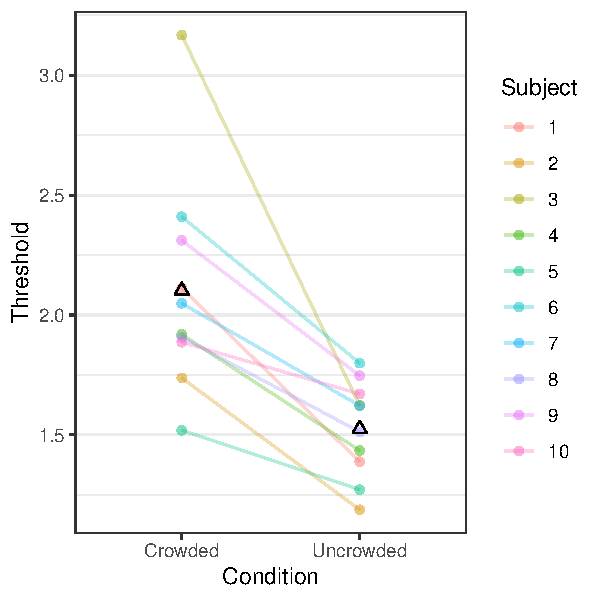
\includegraphics{tutorial_files/figure-latex/unnamed-chunk-9-1} 

}

\caption{Size (in arcminutes) at which threshold performance (62.5\% correct) was reached by crowding condition. Each color shows a separate subject. Black triangles show the predicted outcome of a linear model fit to the data.}\label{fig:unnamed-chunk-9}
\end{figure}

\normalsize

\hypertarget{prepare-for-class}{%
\subsubsection{Prepare for class}\label{prepare-for-class}}

\begin{enumerate}
\def\labelenumi{\arabic{enumi}.}
\tightlist
\item
  Why does the model predict only two different values for the outcome
  variable?
\item
  How would you calculate the epsilon/residual for each observation from
  this data? (Try it)
\item
  How could you calculate the residual sum of squares for this model
  from this data? (Try it)
\item
  We obtain the straightforward interpretation of the ConditionCrowded
  estimate only because we coded the treatment condition as 1, rather
  than, e.g., as 2. What would happen if we coded the treatment
  condition as 2 (and the reference condition still as 0)? Would our
  estimate for the coefficient for ConditionCrowded change? What about
  the estimate of the intercept? Why? (Much of this can be answered by
  trying to change the coding)
\item
  Would the predicted/fitted values of the model change if we change the
  coding to 2 vs.~0? Why?
\end{enumerate}

\hypertarget{questions-for-discussion-in-class}{%
\subsubsection{Questions for discussion in
class}\label{questions-for-discussion-in-class}}

\begin{enumerate}
\def\labelenumi{\arabic{enumi}.}
\setcounter{enumi}{5}
\tightlist
\item
  How could you calculate the \(R^2\) value shown as part of the model
  output from just the predicted/fitted values and the original data?
  (cf.~James et al., 2013, p.~70-71)
\end{enumerate}

\hypertarget{effectdeviationsumanova-coding}{%
\subsection{Effect/deviation/sum/anova-coding}\label{effectdeviationsumanova-coding}}

While treatment-coding is the default in the regression world, it is
actually rarely used in experimental psychology, brain imaging, or
related fields that use factorial/balanced designs. Rather, we typically
code our data in a different way, because it changes the interpretation
of the intercept in ways that researchers that are used to ANOVA tend to
find more intuitive. This alternative is called
effect/deviation/sum/anova-coding:

\footnotesize

\begin{verbatim}
          Crowded.vs.Uncrowded
Crowded                    0.5
Uncrowded                 -0.5
\end{verbatim}

\normalsize

With this change in contrast, the model matrix also changes:

\footnotesize

\begin{Shaded}
\begin{Highlighting}[]
\KeywordTok{model.matrix}\NormalTok{( }\OperatorTok{~}\StringTok{ }\DecValTok{1} \OperatorTok{+}\StringTok{ }\NormalTok{Condition, }\DataTypeTok{data =}\NormalTok{ d)}
\end{Highlighting}
\end{Shaded}

\begin{verbatim}
   (Intercept) ConditionCrowded.vs.Uncrowded
1            1                          -0.5
2            1                          -0.5
3            1                          -0.5
4            1                          -0.5
5            1                          -0.5
6            1                          -0.5
7            1                          -0.5
8            1                          -0.5
9            1                          -0.5
10           1                          -0.5
11           1                           0.5
12           1                           0.5
13           1                           0.5
14           1                           0.5
15           1                           0.5
16           1                           0.5
17           1                           0.5
18           1                           0.5
19           1                           0.5
20           1                           0.5
attr(,"assign")
[1] 0 1
attr(,"contrasts")
attr(,"contrasts")$Condition
          Crowded.vs.Uncrowded
Crowded                    0.5
Uncrowded                 -0.5
\end{verbatim}

\normalsize

Let's refit the model with this newly coded factor:

\footnotesize

\begin{verbatim}

Call:
lm(formula = Threshold ~ 1 + Condition, data = d)

Residuals:
     Min       1Q   Median       3Q      Max 
-0.58347 -0.19997 -0.03302  0.16157  1.06575 

Coefficients:
                              Estimate Std. Error t value Pr(>|t|)    
(Intercept)                    1.81354    0.07886  22.997 8.54e-15 ***
ConditionCrowded.vs.Uncrowded  0.57672    0.15772   3.657   0.0018 ** 
---
Signif. codes:  0 '***' 0.001 '**' 0.01 '*' 0.05 '.' 0.1 ' ' 1

Residual standard error: 0.3527 on 18 degrees of freedom
Multiple R-squared:  0.4262,    Adjusted R-squared:  0.3943 
F-statistic: 13.37 on 1 and 18 DF,  p-value: 0.001805
\end{verbatim}

\normalsize

In this deviation-coded model:

\begin{itemize}
\tightlist
\item
  the intercept estimate is now the predicted \emph{overall mean} of the
  outcome.
\item
  the estimate for the coefficient of Condition is the predicted
  difference between the two conditions.
\item
  the two conditions means are described as the sum of the intercept
  estimate +/- .5-times the estimate for the coefficient of Condition.
\end{itemize}

Why do researchers used to ANOVA find this more intuitive? You'll
sometimes here that it's nice that the intercept now corresponds to the
mean, but the true convenience of this coding scheme will become
apparent once we consider interactions below. It is under
deviation-coding, that we can talk about \emph{main effects} and
\emph{interactions} in the same sense as in an ANOVA. That's presumably
also why some people call this coding scheme anova-coding. We'll get to
that. But first some questions.

\hypertarget{prepare-for-class-1}{%
\subsubsection{Prepare for class}\label{prepare-for-class-1}}

\begin{enumerate}
\def\labelenumi{\arabic{enumi}.}
\tightlist
\item
  What happens if we double the values we assign to each of the two
  deviation-coded conditions, i.e., if we use 1 vs.~-1 instead of .5
  vs.~-.5? What if we set them to -1000 vs.~1000? What changes and what
  doesn't? Why? (Try it)
\end{enumerate}

\footnotesize

\begin{Shaded}
\begin{Highlighting}[]
\KeywordTok{contrasts}\NormalTok{(d}\OperatorTok{$}\NormalTok{Condition) =}\StringTok{ }\KeywordTok{cbind}\NormalTok{(}\StringTok{"Crowded vs. Uncrowded"}\NormalTok{ =}\StringTok{ }\KeywordTok{c}\NormalTok{(}\DecValTok{1}\NormalTok{,}\OperatorTok{-}\DecValTok{1}\NormalTok{))}
\end{Highlighting}
\end{Shaded}

\normalsize

\begin{enumerate}
\def\labelenumi{\arabic{enumi}.}
\setcounter{enumi}{1}
\tightlist
\item
  Are the predicted/fitted values of any of these deviation-coded models
  different from each other? (Try it)
\item
  Are the predicted/fitted values of any of these deviation-coded models
  different from the treatment-coded model presented in the previous
  section? Why?
\end{enumerate}

\hypertarget{discussion-questions-for-class}{%
\subsubsection{Discussion questions for
class}\label{discussion-questions-for-class}}

\begin{enumerate}
\def\labelenumi{\arabic{enumi}.}
\setcounter{enumi}{3}
\tightlist
\item
  We obtain the intuitive interpretation of the intercept (as the
  predicted grand mean of the data) only because the data is \ldots{}
  what? (recall that the intercept is \emph{always} the predicted value
  for the case when all other terms add up to zero). Conveniently, most
  data sets obtained from psychological experiments have the same
  property we are looking for here---either exactly or at least
  approximately (after exclusions).
\end{enumerate}

\hypertarget{writing-up-results-1}{%
\subsection{Writing up results}\label{writing-up-results-1}}

How would we write up, for example, the deviation-coded model. There
are, of course, about as many difference preferences as they are
researchers, and so you will find conflicting advice. But generally, it
will be helpful if you are clear about all of the following:

\begin{itemize}
\tightlist
\item
  What model you used
\item
  What predictors you considered (incl.~those that you did not include
  in the final model, cf.~debate about \emph{researchers' degrees of
  freedom})
\item
  How you coded the outcome (e.g., what unit is the outcome in; without
  this information, readers cannot determine the size of effects or
  interpret them on the original scale)
\item
  How you coded predictors (without this information, readers cannot
  even determine in which \emph{direction} the effect is!)
\item
  What steps (if any) were taken to ascertain the validity of the model
  (see, e.g., model evaluation in Gelman \& Hill, 2007, Section 3.7).
  This is arguably less important if you study a well-known phenomenon
  that has been analyzed with this method many times, and for which you
  have data that is a) balanced with regard to the predictors in the
  model, and b) has many observations relative to the number of
  predictors in the model.
\end{itemize}

When reporting results, I recommend you provide both the relevant
statistics (coefficient estimates, \(p\)-values, etc.), and a
descriptive interpretation of that result in non-technical
language---but we careful to avoid language that is wrong (see, e.g.,
section on interactions for some examples). Finally, for any non-trivial
model, I highly recommend the use of a summary table of the model and
visualization of the \emph{empirical} distribution of the data
(potentially, while \emph{also} showing the model's predictions). The
latter helps readers not familiar with the analysis approach to
understand your results.

Here is a rather detailed write-up for the model with the
deviation-coded condition variable. In many scenarios (e.g., if the
units of the outcome variable are not necessarily informative), you
might decide to provide less detail:

\color{lightgray}

We analyzed the data with a linear regression, using the function
\texttt{lm} from the \texttt{base} package (citation with version) of
the software \texttt{R} (citation with version). We calculated each
subject's mean thresholds for the crowded and uncrowded condition. These
20 threshold values were regressed against condition (deviation-coded:
.5 = \emph{crowded} vs.~-.5 = \emph{uncrowded}). We found a
statistically significant main effect of condition
(\(\widehat{\beta}=.576, t=3.657, p<.01\)), so that subjects reached
threshold performance at a size that was about half an arcminute larger
in the crowded condition (mean = 2.102), compared to the uncrowded
condition (mean = 1.525). \color{black}

\hypertarget{combining-factors-and-continuous-predictors}{%
\section{Combining factors and continuous
predictors}\label{combining-factors-and-continuous-predictors}}

Now that we know how to code factors (or at least binary factor), we can
combine continuous and categorical predictors in our model. We first
show a simple `additive' model, in which we assume that the effects of
the categorical and continuous predictors are additive. Then we consider
a model that also contains an interaction, allowing the two effects to
be more or less than additive. \textbf{The models presented here merely
serve the purpose of illustrating how we can fit, analyze, and interpret
models with continuous and categorical predictors. The one degree of
freedom we have in our model so far (Condition) already puts as at the
maximum of the recommended degrees of freedom for 20 data points.}
Including additional parameters, as we do below, increases the risk of
overfitting the model to the data.

\hypertarget{do-both-the-diffusion-constant-and-the-crowdedness-condition-affect-threshold-performance}{%
\subsection{Do both the diffusion constant and the crowdedness condition
affect threshold
performance?}\label{do-both-the-diffusion-constant-and-the-crowdedness-condition-affect-threshold-performance}}

For example, let's test the effects of both Condition and
DiffusionConstant. For simplicity's sake, we continue to use deviation
coding for Condition:

\[ Threshold \sim 1 + Condition + DiffusionConstant \] What happens when
we include both of these predictors in the LM?

\footnotesize

\begin{verbatim}

Call:
lm(formula = Threshold ~ 1 + Condition + DiffusionConstant, data = d)

Residuals:
     Min       1Q   Median       3Q      Max 
-0.29652 -0.13259 -0.04913  0.10420  0.44403 

Coefficients:
                               Estimate Std. Error t value Pr(>|t|)    
(Intercept)                    1.260450   0.097333  12.950 3.11e-10 ***
ConditionCrowded vs. Uncrowded 0.431381   0.091055   4.738  0.00019 ***
DiffusionConstant              0.034632   0.005434   6.373 6.94e-06 ***
---
Signif. codes:  0 '***' 0.001 '**' 0.01 '*' 0.05 '.' 0.1 ' ' 1

Residual standard error: 0.1971 on 17 degrees of freedom
Multiple R-squared:  0.8307,    Adjusted R-squared:  0.8108 
F-statistic: 41.71 on 2 and 17 DF,  p-value: 2.775e-07
\end{verbatim}

\normalsize

Right away, we can see that the diffusion constant seems to account for
a \emph{lot} of additional variability in the model: the \(R^2\) of the
model is almost twice as large as the one we obtained when only
considering condition. The output of the regression also tell us that
both of the predictors have statistically significant effects on
subjects' threshold performance. We can visualize the data and the
model's predictions together:

\footnotesize

\begin{figure}

{\centering 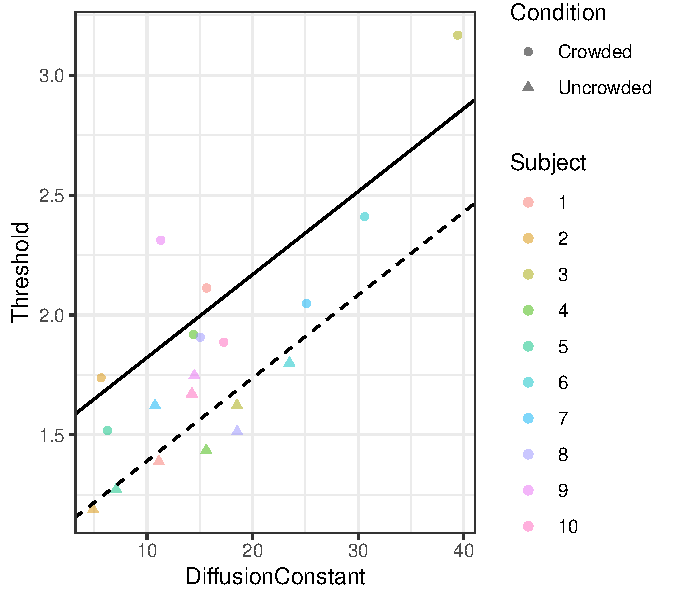
\includegraphics{tutorial_files/figure-latex/unnamed-chunk-15-1} 

}

\caption{Size (in arcminutes) at which threshold performance (62.5\% correct) was reached by diffusion constant and crowding condition. Each color shows a separate subject. Black lines show the predicted outcome of a linear model fit to the data.}\label{fig:unnamed-chunk-15}
\end{figure}

\normalsize

\hypertarget{write-up}{%
\subsubsection{Write-up}\label{write-up}}

Here's a somewhat less detailed write-up for our two-predictor model,
building on the example provided above:

\color{lightgray}

We analyzed the data with a linear regression, using the function
\texttt{lm} from the \texttt{base} package (citation with version) of
the software \texttt{R} (citation with version). We calculated each
subject's mean thresholds for the crowded and uncrowded condition. These
20 threshold values were regressed against condition (deviation-coded:
.5 = \emph{crowded} vs.~-.5 = \emph{uncrowded}) \textbf{and the
diffusion constant}. We found a statistically significant effect of
condition (\(\widehat{\beta}=.431, t=4.738, p<.01\)), so that subjects
reach threshold performance at larger sizes in the crowded condition,
compared to the uncrowded condition. \textbf{We also found a
statistically significant effect of the diffusion constant
(\(\widehat{\beta}=.035, t=6.373, p<.01\)), so that larger diffusion
constants required larger sizes to achieve threshold performance.}
\color{black}

\hypertarget{prepare-for-class-2}{%
\subsubsection{Prepare for class}\label{prepare-for-class-2}}

\begin{enumerate}
\def\labelenumi{\arabic{enumi}.}
\tightlist
\item
  Notice how that the intercept estimate in this model is not the same
  as in the model that only contains Condition as a predictor. That also
  means that the intercept no longer represents the prediction for the
  grand mean of the outcome. Was that inevitable? Can you think of a
  scenario in which the inclusion of the additional predictor
  (DiffusionConstant) would \emph{not} change the intercept estimate?
  (Recall that the intercept always is the model's prediction when all
  other terms of the model add to 0.) If you get stuck on this question,
  it will get resolved in the next section, but think about it before
  you read on.
\item
  The coefficient estimate for Condition has changed. Specifically, it
  is now somewhat smaller (.431 vs.~.576). What do you make out this?
  Does it tell you something about the relation between the two
  \emph{predictors} (Condition and DiffusionConstant)?
\item
  What is an intuitive geometric interpretation of this model? The
  effect of a single continuous predictor (DiffusionConstant) is
  described by the intercept and slope. So what does the present model
  result in? (If you get stuck in thinking about this, re-read Gelman \&
  Hill, 2007, p.~31-33).
\end{enumerate}

\hypertarget{discussion-questions-for-class-1}{%
\subsubsection{Discussion questions for
class}\label{discussion-questions-for-class-1}}

\begin{enumerate}
\def\labelenumi{\arabic{enumi}.}
\setcounter{enumi}{3}
\tightlist
\item
  Can we conclude from this model, and the fact that the two predictors
  are both significant, that the two effects are additive? Why or why
  not?
\item
  Can we conclude that DiffusionConstant has an effect in both
  crowdedness conditions? Why or why not?
\item
  Can we conclude that DiffusionConstant had an independent effect
  beyond condition? Why or why not?
\end{enumerate}

\hypertarget{intermezzo-centering-continuous-predictors}{%
\section{Intermezzo: centering continuous
predictors}\label{intermezzo-centering-continuous-predictors}}

Recall that the intercept estimate changed once we added the
DiffusionConstant as a predictor to the LM. As we've already covered,
the intercept always gives us the prediction when all other terms in the
model add up to 0 (because, if \(\beta_1 x_1 + ... + beta_k x_k = 0\)
then the LM predicts that \(E(y) = \beta_0\)). Partly for this reason,
it is often recommended that all predictors in the model are
\emph{centered}. Since the mean of a centered predictor \(x_i\) is 0
(i.e., \(E(x_i) = 0\)), the average of the term \(\beta_i x_i\) is also
0. So if \emph{all} predictors in a model are centered, then
\(\forall i: \beta_i x_i = 0 \Rightarrow \Sigma_{i=1}^k \beta_i x_i = 0 \Rightarrow E(y) = \beta_0\).

For data that is balanced with regard to a factor (e.g., Condition),
deviation-coding results in a centered predictor. For example, for the
deviation-coded model introduced above, we coded the crowded condition
as .5 and the uncrowded condition as -.5. If both conditions appear
equally often in the data (as they do), then the average of the
implicitly created numerical predictor that results from this coding is
0.

But what about the continuous predictor in our model. DiffusionConstant
does not have a mean of zero:

\footnotesize

\begin{Shaded}
\begin{Highlighting}[]
\KeywordTok{round}\NormalTok{(}\KeywordTok{mean}\NormalTok{(d}\OperatorTok{$}\NormalTok{DiffusionConstant), }\DecValTok{5}\NormalTok{)}
\end{Highlighting}
\end{Shaded}

\begin{verbatim}
[1] 15.97013
\end{verbatim}

\normalsize

In the combined model from the previous section, the intercept estimate
thus corresponds to the threshold value that is expected when the
diffusion constant is 0, which it never is because all values of the
diffusion constant are positive:

\footnotesize

\begin{Shaded}
\begin{Highlighting}[]
\KeywordTok{range}\NormalTok{(d}\OperatorTok{$}\NormalTok{DiffusionConstant)}
\end{Highlighting}
\end{Shaded}

\begin{verbatim}
[1]  4.893119 39.431606
\end{verbatim}

\normalsize

Once we center diffusion constant by subtracting its mean from each of
its values, the new mean of the centered diffusion constant
(DiffusionConstant\_c) is 0:

\footnotesize

\begin{Shaded}
\begin{Highlighting}[]
\NormalTok{d }\OperatorTok
\StringTok{  }\KeywordTok{mutate}\NormalTok{(}\KeywordTok{across}\NormalTok{(}\KeywordTok{where}\NormalTok{(is.numeric), }\KeywordTok{list}\NormalTok{(}\StringTok{"c"}\NormalTok{ =}\StringTok{ }\ControlFlowTok{function}\NormalTok{(x) x }\OperatorTok{-}\StringTok{ }\KeywordTok{mean}\NormalTok{(x))))}
\KeywordTok{round}\NormalTok{(}\KeywordTok{mean}\NormalTok{(d}\OperatorTok{$}\NormalTok{DiffusionConstant_c), }\DecValTok{5}\NormalTok{)}
\end{Highlighting}
\end{Shaded}

\begin{verbatim}
[1] 0
\end{verbatim}

\normalsize

When we re-fit the combined LM from the previous section with the new
centered diffusion constant, the \textbf{intercept estimate now again
predicts the overall mean threshold}:

\footnotesize

\begin{verbatim}

Call:
lm(formula = Threshold ~ 1 + Condition + DiffusionConstant_c, 
    data = d)

Residuals:
     Min       1Q   Median       3Q      Max 
-0.29652 -0.13259 -0.04913  0.10420  0.44403 

Coefficients:
                               Estimate Std. Error t value Pr(>|t|)    
(Intercept)                    1.813535   0.044077  41.145  < 2e-16 ***
ConditionCrowded vs. Uncrowded 0.431381   0.091055   4.738  0.00019 ***
DiffusionConstant_c            0.034632   0.005434   6.373 6.94e-06 ***
---
Signif. codes:  0 '***' 0.001 '**' 0.01 '*' 0.05 '.' 0.1 ' ' 1

Residual standard error: 0.1971 on 17 degrees of freedom
Multiple R-squared:  0.8307,    Adjusted R-squared:  0.8108 
F-statistic: 41.71 on 2 and 17 DF,  p-value: 2.775e-07
\end{verbatim}

\normalsize

This---that the intercept estimates is the predicted grand mean of the
outcome---will always be the case, no matter how many predictors we have
in the model.

\textbf{Note further that centering does \emph{not} affect the slope
estimates for the other effects in the model.} Neither does it affect
the standard error estimates of those slopes (or \(t\) statistics or
\(p\)-value). Removing the mean from a predictor is a linear
transformation does not affect the best-fitting slope of that predictor
in predicting the outcome of an LM. Neither does centering affect the
predicted/fitted values of the LM (you can compare the 20
predicted/fitted values for the combined model before and after
centering DiffusionConstant). The same holds, of course, for the
residuals, the \(R^2\), the adusted \(R^2\) and similar measures.

This will \emph{not} always be the case. In the next section, for
example, we will see that centering can change the standard error (and
thus \(t\) statistic and \(p\)-value) for an interaction. More
generally, centering can affect the the standard error when the removal
of the mean from each variable changes the correlations between
predictors (we we will return to the issue of correlations between
predictors in future meetings).

\hypertarget{interactions-between-factors-and-continuous-predictors}{%
\section{Interactions between factors and continuous
predictors}\label{interactions-between-factors-and-continuous-predictors}}

Next, we expand the analysis further. We remove the additivity
assumption. Or rather, the addidivity assumption still holds but we
expand the model in a way that we are not assuming the our two
predictors are additive. This is done by including an interaction
between the two predictors. Here I show this for the case of one
continuous predictor (DiffusionConstant) and one binary categorical
predictor (Condition), but the same logic extends to interactions
between multiple continuous or multiple categorical predictors, as well
as interactions between interactions (e.g., three-way interactions,
etc.). Like for the remainder of this tutorial, we focus on the type of
planned analysis typical for (or at least the idea of) experimental
psychology. For that reason, we do not discuss considerations about when
we should even consider an interaction (but see, for example, Harrell,
2001 for insightful discussion, as well as Gelman \& Hill, 2007,
p.~36).\footnote{The short of those considerations is that introducing
  additional complexity (degrees of freedom) increases the risk of
  overfitting to the data, and with it the risk of spurious/unreliable
  conclusions. It is thus advisable to include additional complexity in
  the model only if is is motivated theoretically, by previous work, or
  other a priori considerations. Another specific recommendation you'll
  see often is to only include interactions if all their components are
  also included in the model, unless there is a good theoretical reason
  to do otherwise. These recommendations are not specific to the LM.}

For the case of one continuous and one categorical predictor, the
geometric interpretation of the model is that we now allow the two lines
(corresponding to the continuous predictor's effect at the two levels of
the categorical predictor) to not be parallel. And our question of
whether the interaction is \emph{significant} becomes the question
whether the difference in the slope of the two lines is statistically
different from zero.

We can ask this question by adding a new predictor to the model that is
the \emph{product} of the two predictors (cf.~Gelman \& Hill, 2007,
p.~34-36; James et al., 2013, p.~87-90). We then ask whether this new
predictor has a non-zero effect, i.e., we ask whether the coefficient
for this new predictor is different from zero. In R, the regression
formula for this model is written as (where the colon is the interaction
operator):

\[ Threshold \sim 1 + Condition + DiffusionConstant + Condition:DiffusionConstant\]

which essentially runs the following model (where I is the identity
operator, which return x for x):

\[ Threshold \sim 1 + Condition + DiffusionConstant + I(Condition * DiffusionConstant)\]

or shorter (where X1 * X2 is a shorthand for the full-factorial
combination of X1 and X2):

\[ Threshold \sim 1 + Condition*DiffusionConstant\]

Just like, e.g., factor coding implicit creates an additional numerical
variable that encodes the factor's information, the interaction operator
implicitly creates a new variable in our data that is the product if the
(numerically coded) factor Condition and the continuous predictor
DiffusionConstant. To see this, we again look at the model matrix:

With this change in contrast, the model matrix also changes:

\footnotesize

\begin{Shaded}
\begin{Highlighting}[]
\KeywordTok{model.matrix}\NormalTok{( }\OperatorTok{~}\StringTok{ }\DecValTok{1} \OperatorTok{+}\StringTok{ }\NormalTok{Condition }\OperatorTok{*}\StringTok{ }\NormalTok{DiffusionConstant, }\DataTypeTok{data =}\NormalTok{ d)}
\end{Highlighting}
\end{Shaded}

\begin{verbatim}
   (Intercept) ConditionCrowded vs. Uncrowded DiffusionConstant ConditionCrowded vs. Uncrowded:DiffusionConstant
1            1                           -0.5         11.123343                                        -5.561671
2            1                           -0.5          4.893119                                        -2.446560
3            1                           -0.5         18.518145                                        -9.259072
4            1                           -0.5         15.609822                                        -7.804911
5            1                           -0.5          7.069902                                        -3.534951
6            1                           -0.5         23.487701                                       -11.743851
7            1                           -0.5         10.750472                                        -5.375236
8            1                           -0.5         18.541809                                        -9.270905
9            1                           -0.5         14.479893                                        -7.239946
10           1                           -0.5         14.243763                                        -7.121881
11           1                            0.5         15.638986                                         7.819493
12           1                            0.5          5.644884                                         2.822442
13           1                            0.5         39.431606                                        19.715803
14           1                            0.5         14.408659                                         7.204329
15           1                            0.5          6.249123                                         3.124562
16           1                            0.5         30.619534                                        15.309767
17           1                            0.5         25.096704                                        12.548352
18           1                            0.5         15.031910                                         7.515955
19           1                            0.5         11.302197                                         5.651099
20           1                            0.5         17.261093                                         8.630547
attr(,"assign")
[1] 0 1 2 3
attr(,"contrasts")
attr(,"contrasts")$Condition
          Crowded vs. Uncrowded
Crowded                     0.5
Uncrowded                  -0.5
\end{verbatim}

\normalsize

\hypertarget{do-the-effects-of-condition-and-difficusion-constant-interact}{%
\subsection{Do the effects of condition and difficusion constant
interact?}\label{do-the-effects-of-condition-and-difficusion-constant-interact}}

Now we can fit the new LM with the interaction, and look at the summary
of results. We will use the centered DiffusionConstant for this
model---i.e., we'll fit the model \$ Threshold \sim 1 +
Condition*DiffusionConstant\_c\$. For this model, we can refer to the
effect of condition as the ``\emph{main} effect'' of condition (roughyl
speaking, the overall, or mean, effect of condition). If we didn't
center the diffusion constant---and more generally, if there were other
uncentered variables in the model---the effect of of condition would not
be conventionally referred to as main effect.

\footnotesize

\begin{verbatim}

Call:
lm(formula = Threshold ~ 1 + Condition * DiffusionConstant_c, 
    data = d)

Residuals:
     Min       1Q   Median       3Q      Max 
-0.30964 -0.14039 -0.05505  0.10824  0.45666 

Coefficients:
                                                   Estimate Std. Error t value Pr(>|t|)    
(Intercept)                                        1.804444   0.047022  38.374  < 2e-16 ***
ConditionCrowded vs. Uncrowded                     0.441727   0.094044   4.697 0.000242 ***
DiffusionConstant_c                                0.032167   0.006725   4.783 0.000203 ***
ConditionCrowded vs. Uncrowded:DiffusionConstant_c 0.008665   0.013449   0.644 0.528534    
---
Signif. codes:  0 '***' 0.001 '**' 0.01 '*' 0.05 '.' 0.1 ' ' 1

Residual standard error: 0.2006 on 16 degrees of freedom
Multiple R-squared:  0.835, Adjusted R-squared:  0.8041 
F-statistic: 26.99 on 3 and 16 DF,  p-value: 1.695e-06
\end{verbatim}

\normalsize

The first thing we can notice is that the \(R^2\) of the model has
barely increased. In other words, adding the interaction doesn't explain
much more variance in the outcome. Indeed, the adjusted \(R^2\) (which
is the \(R^2\) corrected for the complexity of the model) has
\emph{de}creased. With this in mind, it is not surprising that the
interaction does not have a significant effect. In short, we cannot
reject the null hypothesis that the effect of the diffusion constant on
the threshold is identical for crowded and uncrowded condition. This is
also in line with a visualization of the data and the model:

\footnotesize

\begin{figure}

{\centering 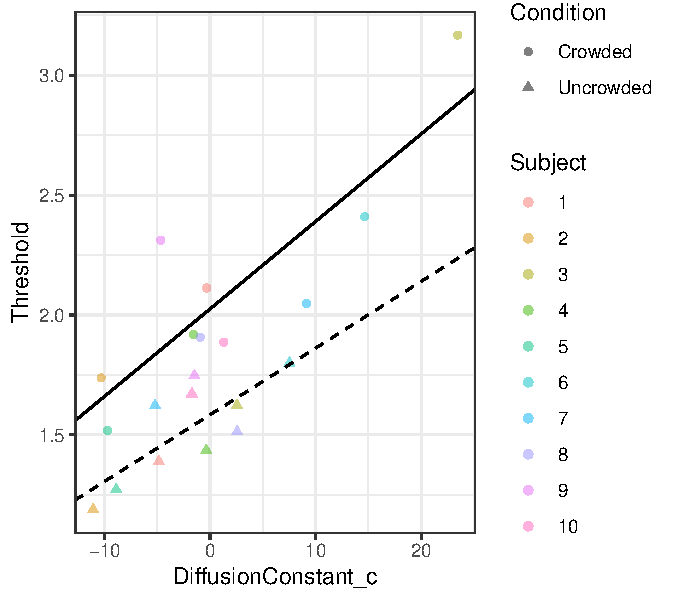
\includegraphics{tutorial_files/figure-latex/unnamed-chunk-22-1} 

}

\caption{Size (in arcminutes) at which threshold performance (62.5\% correct) was reached by diffusion constant (centered) and crowding condition. Each color shows a separate subject. Black lines show the predicted outcome of a linear model fit to the data.}\label{fig:unnamed-chunk-22}
\end{figure}

\normalsize

In the LM with the interaction, the main effect of diffusion constant is
the \emph{average} effect of the diffusion constant across the two
conditions (because we effect-coded and thus centered condition). The
main effect of condition is the \emph{average} across all values of the
diffusion constant (because we centered the diffusion constant, so that
the effect of condition is the predicted distance between the lines when
the centered diffusion constant is zero, i.e., at the mean of the
diffusion constant). The interaction tells us how much the slope of the
diffusion constant differs between the conditions. Specifically, the
slope of the diffusion constant for the crowded condition is predicted
to be + 0.008665 * 0.05 = + 0.0043325 larger than the main effect of the
diffusion constant (0.032167 + 0.0043325), whereas the slope of the
diffusion constant for the uncrowded condition is predicted to be +
0.008665 * -0.05 = - 0.0043325 smaller than the main effect of the
diffusion constant (0.032167 - 0.0043325).

Note also that the intercept estimate in the interaction model is not
identical to the one from the combined model. This seems to contradict
what we learned above, that the intercept estimate is the model's
prediction for the grand mean if all predictors are centered. Note,
however, that we did not center the interaction and, indeed, the mean of
the product of condition and DiffusionConstant is \emph{not} 0, but
rather 1.049. There's thus no contradiction to the generalization that
the intercept is the model's predicted overall mean outcome when all
variables are centered.\footnote{Since the diffusion constant is not a
  variable that we controlled directly by our design, it can have
  different means for the two conditions even after centering it, and
  indeed it does (centering only guarantees that the \emph{overall} mean
  of the diffusion constant is 0): In other words, the diffusion
  constant is itself affected by the condition and, as a consequence,
  condition and DiffusionConstant are correlated. Here we don't explore
  this further, but we will return to questions about collinearity later
  in the semester.}

\hypertarget{prepare-for-class-3}{%
\subsubsection{Prepare for class}\label{prepare-for-class-3}}

\begin{enumerate}
\def\labelenumi{\arabic{enumi}.}
\tightlist
\item
  On Figure 3, draw line segment that correspond to the intercept.
\item
  On Figure 3, draw line segment that correspond to the effect of
  condition.
\item
  Calculate the slope for the crowded condition from the model output
  shown above.
\item
  What's a geometric interpretation of an interaction between two
  \emph{continuous} predictors (x1 and x2)? For this it might be helpful
  to first think about the geometric interpretation of two additive
  continuous predictors (a plane over x1 and x2, the height of which is
  given along the third axis, y)
\item
  True or false? Since the interaction does not have a significant
  effect, we can safely remove it from the model.
\end{enumerate}

\hypertarget{discussion-questions-for-class-2}{%
\subsubsection{Discussion questions for
class}\label{discussion-questions-for-class-2}}

\begin{enumerate}
\def\labelenumi{\arabic{enumi}.}
\setcounter{enumi}{5}
\tightlist
\item
  True or false? Now that we know that the slope of diffusion constant
  does not significantly differ between the two crowdedness conditions,
  and given that the effect of diffusion constant was significant, we
  can conclude that both conditions exhibit a significant effect of the
  diffusion constant.
\item
  True or false? If we had found a significant interaction between
  condition and diffusion constant, we could have concluded that the
  effect of conclusion constant goes in opposite directions for the two
  conditions?
\item
  When we fit the same interaction model with the uncentered diffusion
  constant instead, we get a seemingly conflicting result, where
  condition does not longer have a significant effect. Why is that the
  case? Is this result really conflicting? (The figure might help. Hint:
  draw the line segments corresponding to the effect of condition in
  this new interaction model.)
\end{enumerate}

\footnotesize

\begin{verbatim}

Call:
lm(formula = Threshold ~ 1 + Condition * DiffusionConstant, data = d)

Residuals:
     Min       1Q   Median       3Q      Max 
-0.30964 -0.14039 -0.05505  0.10824  0.45666 

Coefficients:
                                                 Estimate Std. Error t value Pr(>|t|)    
(Intercept)                                      1.290728   0.109636  11.773 2.71e-09 ***
ConditionCrowded vs. Uncrowded                   0.303347   0.219271   1.383 0.185531    
DiffusionConstant                                0.032167   0.006725   4.783 0.000203 ***
ConditionCrowded vs. Uncrowded:DiffusionConstant 0.008665   0.013449   0.644 0.528534    
---
Signif. codes:  0 '***' 0.001 '**' 0.01 '*' 0.05 '.' 0.1 ' ' 1

Residual standard error: 0.2006 on 16 degrees of freedom
Multiple R-squared:  0.835, Adjusted R-squared:  0.8041 
F-statistic: 26.99 on 3 and 16 DF,  p-value: 1.695e-06
\end{verbatim}

\begin{figure}

{\centering 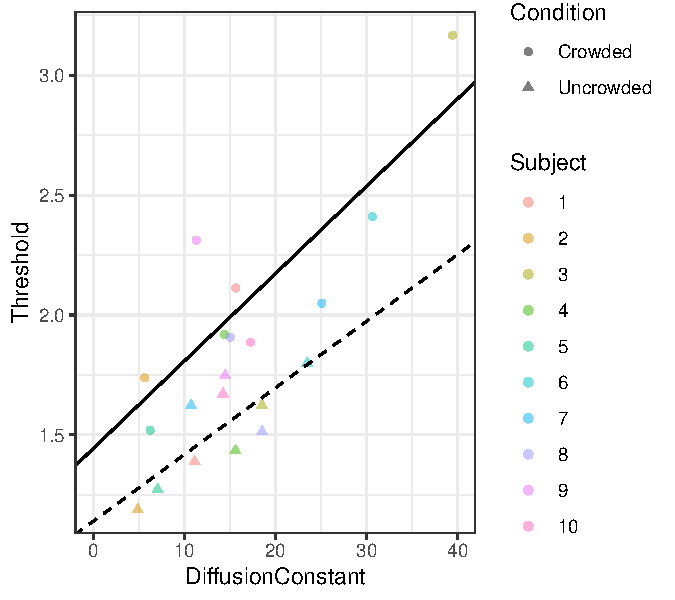
\includegraphics{tutorial_files/figure-latex/unnamed-chunk-23-1} 

}

\caption{Size (in arcminutes) at which threshold performance (62.5\% correct) was reached by diffusion constant (not-centered) and crowding condition. Each color shows a separate subject. Black lines show the predicted outcome of a linear model fit to the data.}\label{fig:unnamed-chunk-23}
\end{figure}

\normalsize

\begin{enumerate}
\def\labelenumi{\arabic{enumi}.}
\tightlist
\item
  Are the predicted/fitted values from this model different from the
  first interaction model we fit above?
\end{enumerate}

\hypertarget{simple-effects}{%
\subsection{Simple effects}\label{simple-effects}}

When we have interactions in our model, we might also want to report the
\emph{simple effects}. For example, for the two-way interaction between
condition and diffusion constant, we might want to report the simple
effect of the diffusion constant for each condition. That's necessary
because a significant interaction between two predictors \(x_1\) and
\(x_2\) only tells us that the effect of \(x_1\) on \(y\) differs
depending on \(x_2\) (or vice versa, that the effect of \(x_2\) on \(y\)
depends on the value of \(x_1\)). For example, for the present case a
significant interaction would have indicated that the slope of diffusion
constant differs between the two crowdedness conditions.

\textbf{However, a signficant interaction does \emph{not} tell us
\emph{how} the interacting effects depends on each other.} For example,
for the present case a significant interaction could indicate that there
is a significant positive relation between the diffusion constant and
threshold in one condition and a significant negative relation in the
other condition; but it could also indicate that there is a significant
positive relation in one condition and a non-significant relation in the
other; or even that the relation is significant and positive in both
conditions but the size of the effect of diffusion constant differs
between condition (and so on). To address which of those scenarios
holds, it is necessary to conduct additional analyses. The standard
approach to that is called simple effect analyses.

In this approach, we do not split the data into the two conditions and
fit separate models (\(Threshold \sim 1 + DiffusionConstant\)) to it.
Rather, we use all of the data we have and simple re-parameterize/recode
the same LM we have already fit to read out the simple effects of
DiffusionConstant at each level of condition. In R, this can be done
with the convenient embedding operator /. Here's the model matrix
resulting from this operator does for the present case:

\footnotesize

\begin{Shaded}
\begin{Highlighting}[]
\KeywordTok{model.matrix}\NormalTok{( }\OperatorTok{~}\StringTok{ }\DecValTok{1} \OperatorTok{+}\StringTok{ }\NormalTok{Condition }\OperatorTok{/}\StringTok{ }\NormalTok{DiffusionConstant_c, }\DataTypeTok{data =}\NormalTok{ d)}
\end{Highlighting}
\end{Shaded}

\begin{verbatim}
   (Intercept) ConditionCrowded vs. Uncrowded ConditionCrowded:DiffusionConstant_c ConditionUncrowded:DiffusionConstant_c
1            1                           -0.5                            0.0000000                              -4.846791
2            1                           -0.5                            0.0000000                             -11.077014
3            1                           -0.5                            0.0000000                               2.548011
4            1                           -0.5                            0.0000000                              -0.360311
5            1                           -0.5                            0.0000000                              -8.900231
6            1                           -0.5                            0.0000000                               7.517568
7            1                           -0.5                            0.0000000                              -5.219661
8            1                           -0.5                            0.0000000                               2.571676
9            1                           -0.5                            0.0000000                              -1.490241
10           1                           -0.5                            0.0000000                              -1.726370
11           1                            0.5                           -0.3311476                               0.000000
12           1                            0.5                          -10.3252492                               0.000000
13           1                            0.5                           23.4614730                               0.000000
14           1                            0.5                           -1.5614743                               0.000000
15           1                            0.5                           -9.7210102                               0.000000
16           1                            0.5                           14.6494003                               0.000000
17           1                            0.5                            9.1265712                               0.000000
18           1                            0.5                           -0.9382233                               0.000000
19           1                            0.5                           -4.6679358                               0.000000
20           1                            0.5                            1.2909599                               0.000000
attr(,"assign")
[1] 0 1 2 2
attr(,"contrasts")
attr(,"contrasts")$Condition
          Crowded vs. Uncrowded
Crowded                     0.5
Uncrowded                  -0.5
\end{verbatim}

\normalsize

and here is the resulting LM:

\footnotesize

\begin{verbatim}

Call:
lm(formula = Threshold ~ 1 + Condition/DiffusionConstant_c, data = d)

Residuals:
     Min       1Q   Median       3Q      Max 
-0.30964 -0.14039 -0.05505  0.10824  0.45666 

Coefficients:
                                       Estimate Std. Error t value Pr(>|t|)    
(Intercept)                            1.804444   0.047022  38.374  < 2e-16 ***
ConditionCrowded vs. Uncrowded         0.441727   0.094044   4.697 0.000242 ***
ConditionCrowded:DiffusionConstant_c   0.036500   0.006243   5.846 2.48e-05 ***
ConditionUncrowded:DiffusionConstant_c 0.027835   0.011912   2.337 0.032790 *  
---
Signif. codes:  0 '***' 0.001 '**' 0.01 '*' 0.05 '.' 0.1 ' ' 1

Residual standard error: 0.2006 on 16 degrees of freedom
Multiple R-squared:  0.835, Adjusted R-squared:  0.8041 
F-statistic: 26.99 on 3 and 16 DF,  p-value: 1.695e-06
\end{verbatim}

\normalsize

This re-parameterization does not change the predicted/fitted responses
of the model (not shown here) or the model fit (\(R^2\), F-statistic,
etc.; shown). But we now are provided with the effect of the diffusion
constant at each level of the condition variable. In this case, we see
that the effect of diffusion constant on the threshold is signficant and
positive in both conditions.

\hypertarget{writing-up-the-analysis-results}{%
\subsection{Writing up the analysis
results}\label{writing-up-the-analysis-results}}

\color{lightgray}

We analyzed the data with a linear regression, using the function
\texttt{lm} from the \texttt{base} package (citation with version) of
the software \texttt{R} (citation with version). We calculated each
subject's mean thresholds for the crowded and uncrowded condition. These
20 threshold values were regressed against condition (deviation-coded:
.5 = \emph{crowded} vs.~-.5 = \emph{uncrowded}), the diffusion constant
\textbf{(centered), and their interaction}. We found a statistically
significant \textbf{main} effect of condition
(\(\widehat{\beta}=.442, t=4.697, p<.01\)), so that subjects reach
threshold performance at larger sizes in the crowded condition, compared
to the uncrowded condition. We also found a statistically significant
effect of the diffusion constant
(\(\widehat{\beta}=.037, t=5.846, p<.01\)), so that larger diffusion
constants required larger sizes to achieve threshold performance.
\textbf{The interaction was not significant
(\(\widehat{\beta} = 0.009, p > .5\)).} \color{black}

\hypertarget{additional-topics-we-can-discuss-in-class}{%
\section{Additional topics we can discuss in
class}\label{additional-topics-we-can-discuss-in-class}}

\hypertarget{coding-of-continuous-predictors}{%
\subsection{Coding of continuous
predictors}\label{coding-of-continuous-predictors}}

\begin{itemize}
\tightlist
\item
  scaling (dividing continuous predictors through the standard
  deviation). Why is this done? What are the pros and cons?
\item
  scaling by dividing through two-times the predictors standard
  deviation (Gelman, 2008). Why is this done?
\item
  non-linear transforms of continuous predictors (log-transforming,
  polynomials)? Why is this done? In what sense does the LM still make a
  linearity assumption? (see also James et al., 2013, p.~90-92)
\end{itemize}

\hypertarget{discussion-questions-for-class-3}{%
\subsubsection{Discussion questions for
class}\label{discussion-questions-for-class-3}}

\begin{itemize}
\tightlist
\item
  Can the predictions of models differ depending on the transform of a
  continuous variable?
\item
  Can the conclusions we draw about effects differ depending on the
  transform of a continuous variable?
\end{itemize}

\hypertarget{coding-of-factors-with-more-than-two-levels}{%
\subsection{Coding of factors with more than two
levels}\label{coding-of-factors-with-more-than-two-levels}}

\footnotesize

\normalsize

\begin{itemize}
\item
  Testing hypotheses about the order of levels (see also James et al.,
  2013, p.~85; a nice summary of various coding schemes and how to make
  your own for R can be found at
  \url{https://stats.idre.ucla.edu/r/library/r-library-contrast-coding-systems-for-categorical-variables/}).
  Here are some examples, using all three levels from the complete
  data---i.e., including the ``fixation'' condition:

  \begin{itemize}
  \tightlist
  \item
    treatment coding
  \end{itemize}
\end{itemize}

\footnotesize

\begin{Shaded}
\begin{Highlighting}[]
\KeywordTok{levels}\NormalTok{(d.all}\OperatorTok{$}\NormalTok{Condition)}
\end{Highlighting}
\end{Shaded}

\begin{verbatim}
[1] "Crowded"   "Fixation"  "Uncrowded"
\end{verbatim}

\begin{Shaded}
\begin{Highlighting}[]
\KeywordTok{contrasts}\NormalTok{(d.all}\OperatorTok{$}\NormalTok{Condition) =}\StringTok{ }\KeywordTok{cbind}\NormalTok{(}
  \StringTok{"C"}\NormalTok{ =}\StringTok{ }\KeywordTok{c}\NormalTok{(}\DecValTok{1}\NormalTok{, }\DecValTok{0}\NormalTok{, }\DecValTok{0}\NormalTok{),}
  \StringTok{"U"}\NormalTok{ =}\StringTok{ }\KeywordTok{c}\NormalTok{(}\DecValTok{0}\NormalTok{, }\DecValTok{0}\NormalTok{, }\DecValTok{1}\NormalTok{))}
\KeywordTok{model.matrix}\NormalTok{( }\OperatorTok{~}\StringTok{ }\DecValTok{1} \OperatorTok{+}\StringTok{ }\NormalTok{Condition }\OperatorTok{*}\StringTok{ }\NormalTok{Speed, }\DataTypeTok{data =}\NormalTok{ d.all)}
\end{Highlighting}
\end{Shaded}

\begin{verbatim}
   (Intercept) ConditionC ConditionU    Speed ConditionC:Speed ConditionU:Speed
1            1          0          0 46.69116          0.00000          0.00000
2            1          0          0 43.29595          0.00000          0.00000
3            1          0          0 43.68241          0.00000          0.00000
4            1          0          0 55.86841          0.00000          0.00000
5            1          0          0 39.47389          0.00000          0.00000
6            1          0          0 58.78746          0.00000          0.00000
7            1          0          0 76.61716          0.00000          0.00000
8            1          0          0 59.59884          0.00000          0.00000
9            1          0          0 73.32543          0.00000          0.00000
10           1          0          1 40.59311          0.00000         40.59311
11           1          0          1 38.04379          0.00000         38.04379
12           1          0          1 37.56311          0.00000         37.56311
13           1          0          1 45.66541          0.00000         45.66541
14           1          0          1 37.08101          0.00000         37.08101
15           1          0          1 45.86108          0.00000         45.86108
16           1          0          1 45.60876          0.00000         45.60876
17           1          0          1 47.35490          0.00000         47.35490
18           1          0          1 48.65061          0.00000         48.65061
19           1          0          1 46.31298          0.00000         46.31298
20           1          1          0 43.56899         43.56899          0.00000
21           1          1          0 43.75154         43.75154          0.00000
22           1          1          0 44.85801         44.85801          0.00000
23           1          1          0 48.58767         48.58767          0.00000
24           1          1          0 34.76737         34.76737          0.00000
25           1          1          0 46.08503         46.08503          0.00000
26           1          1          0 44.43581         44.43581          0.00000
27           1          1          0 47.65966         47.65966          0.00000
28           1          1          0 54.05835         54.05835          0.00000
29           1          1          0 54.57448         54.57448          0.00000
attr(,"assign")
[1] 0 1 1 2 3 3
attr(,"contrasts")
attr(,"contrasts")$Condition
          C U
Crowded   1 0
Fixation  0 0
Uncrowded 0 1
\end{verbatim}

\normalsize

\begin{itemize}
\tightlist
\item
  simple coding
\item
  effect (``anova'') coding
\end{itemize}

\footnotesize

\begin{Shaded}
\begin{Highlighting}[]
\KeywordTok{contrasts}\NormalTok{(d.all}\OperatorTok{$}\NormalTok{Condition) =}\StringTok{ }\KeywordTok{cbind}\NormalTok{(}
  \StringTok{"C.vs.F"}\NormalTok{ =}\StringTok{ }\KeywordTok{c}\NormalTok{(.}\DecValTok{5}\NormalTok{,}\OperatorTok{-}\NormalTok{.}\DecValTok{5}\NormalTok{, }\DecValTok{0}\NormalTok{),}
  \StringTok{"U.vs.F"}\NormalTok{ =}\StringTok{ }\KeywordTok{c}\NormalTok{(}\DecValTok{0}\NormalTok{,}\OperatorTok{-}\NormalTok{.}\DecValTok{5}\NormalTok{, }\FloatTok{.5}\NormalTok{))}
\KeywordTok{model.matrix}\NormalTok{( }\OperatorTok{~}\StringTok{ }\DecValTok{1} \OperatorTok{+}\StringTok{ }\NormalTok{Condition }\OperatorTok{*}\StringTok{ }\NormalTok{Speed, }\DataTypeTok{data =}\NormalTok{ d.all)}
\end{Highlighting}
\end{Shaded}

\begin{verbatim}
   (Intercept) ConditionC.vs.F ConditionU.vs.F    Speed ConditionC.vs.F:Speed ConditionU.vs.F:Speed
1            1            -0.5            -0.5 46.69116             -23.34558             -23.34558
2            1            -0.5            -0.5 43.29595             -21.64798             -21.64798
3            1            -0.5            -0.5 43.68241             -21.84121             -21.84121
4            1            -0.5            -0.5 55.86841             -27.93421             -27.93421
5            1            -0.5            -0.5 39.47389             -19.73694             -19.73694
6            1            -0.5            -0.5 58.78746             -29.39373             -29.39373
7            1            -0.5            -0.5 76.61716             -38.30858             -38.30858
8            1            -0.5            -0.5 59.59884             -29.79942             -29.79942
9            1            -0.5            -0.5 73.32543             -36.66272             -36.66272
10           1             0.0             0.5 40.59311               0.00000              20.29655
11           1             0.0             0.5 38.04379               0.00000              19.02190
12           1             0.0             0.5 37.56311               0.00000              18.78155
13           1             0.0             0.5 45.66541               0.00000              22.83270
14           1             0.0             0.5 37.08101               0.00000              18.54051
15           1             0.0             0.5 45.86108               0.00000              22.93054
16           1             0.0             0.5 45.60876               0.00000              22.80438
17           1             0.0             0.5 47.35490               0.00000              23.67745
18           1             0.0             0.5 48.65061               0.00000              24.32530
19           1             0.0             0.5 46.31298               0.00000              23.15649
20           1             0.5             0.0 43.56899              21.78449               0.00000
21           1             0.5             0.0 43.75154              21.87577               0.00000
22           1             0.5             0.0 44.85801              22.42901               0.00000
23           1             0.5             0.0 48.58767              24.29384               0.00000
24           1             0.5             0.0 34.76737              17.38368               0.00000
25           1             0.5             0.0 46.08503              23.04251               0.00000
26           1             0.5             0.0 44.43581              22.21791               0.00000
27           1             0.5             0.0 47.65966              23.82983               0.00000
28           1             0.5             0.0 54.05835              27.02917               0.00000
29           1             0.5             0.0 54.57448              27.28724               0.00000
attr(,"assign")
[1] 0 1 1 2 3 3
attr(,"contrasts")
attr(,"contrasts")$Condition
          C.vs.F U.vs.F
Crowded      0.5    0.0
Fixation    -0.5   -0.5
Uncrowded    0.0    0.5
\end{verbatim}

\normalsize

\begin{itemize}
\tightlist
\item
  Helmert coding (or reverse Helmert coding)
\end{itemize}

\footnotesize

\begin{verbatim}
   (Intercept) Condition1 Condition2    Speed Condition1:Speed Condition2:Speed
1            1          1         -1 46.69116         46.69116        -46.69116
2            1          1         -1 43.29595         43.29595        -43.29595
3            1          1         -1 43.68241         43.68241        -43.68241
4            1          1         -1 55.86841         55.86841        -55.86841
5            1          1         -1 39.47389         39.47389        -39.47389
6            1          1         -1 58.78746         58.78746        -58.78746
7            1          1         -1 76.61716         76.61716        -76.61716
8            1          1         -1 59.59884         59.59884        -59.59884
9            1          1         -1 73.32543         73.32543        -73.32543
10           1          0          2 40.59311          0.00000         81.18621
11           1          0          2 38.04379          0.00000         76.08759
12           1          0          2 37.56311          0.00000         75.12621
13           1          0          2 45.66541          0.00000         91.33082
14           1          0          2 37.08101          0.00000         74.16202
15           1          0          2 45.86108          0.00000         91.72216
16           1          0          2 45.60876          0.00000         91.21752
17           1          0          2 47.35490          0.00000         94.70980
18           1          0          2 48.65061          0.00000         97.30121
19           1          0          2 46.31298          0.00000         92.62596
20           1         -1         -1 43.56899        -43.56899        -43.56899
21           1         -1         -1 43.75154        -43.75154        -43.75154
22           1         -1         -1 44.85801        -44.85801        -44.85801
23           1         -1         -1 48.58767        -48.58767        -48.58767
24           1         -1         -1 34.76737        -34.76737        -34.76737
25           1         -1         -1 46.08503        -46.08503        -46.08503
26           1         -1         -1 44.43581        -44.43581        -44.43581
27           1         -1         -1 47.65966        -47.65966        -47.65966
28           1         -1         -1 54.05835        -54.05835        -54.05835
29           1         -1         -1 54.57448        -54.57448        -54.57448
attr(,"assign")
[1] 0 1 1 2 3 3
attr(,"contrasts")
attr(,"contrasts")$Condition
          [,1] [,2]
Crowded     -1   -1
Fixation     1   -1
Uncrowded    0    2
\end{verbatim}

\normalsize + sliding difference coding (forward/backward) + polynomial
coding (or orthogonal polynomial coding)

\footnotesize

\begin{verbatim}
   (Intercept)   Condition.L Condition.Q    Speed Condition.L:Speed Condition.Q:Speed
1            1 -7.850462e-17  -0.8164966 46.69116     -3.665472e-15         -38.12317
2            1 -7.850462e-17  -0.8164966 43.29595     -3.398932e-15         -35.35100
3            1 -7.850462e-17  -0.8164966 43.68241     -3.429271e-15         -35.66654
4            1 -7.850462e-17  -0.8164966 55.86841     -4.385928e-15         -45.61637
5            1 -7.850462e-17  -0.8164966 39.47389     -3.098883e-15         -32.23029
6            1 -7.850462e-17  -0.8164966 58.78746     -4.615087e-15         -47.99976
7            1 -7.850462e-17  -0.8164966 76.61716     -6.014801e-15         -62.55765
8            1 -7.850462e-17  -0.8164966 59.59884     -4.678784e-15         -48.66225
9            1 -7.850462e-17  -0.8164966 73.32543     -5.756385e-15         -59.86996
10           1  7.071068e-01   0.4082483 40.59311      2.870366e+01          16.57207
11           1  7.071068e-01   0.4082483 38.04379      2.690102e+01          15.53131
12           1  7.071068e-01   0.4082483 37.56311      2.656113e+01          15.33507
13           1  7.071068e-01   0.4082483 45.66541      3.229032e+01          18.64282
14           1  7.071068e-01   0.4082483 37.08101      2.622023e+01          15.13826
15           1  7.071068e-01   0.4082483 45.86108      3.242868e+01          18.72271
16           1  7.071068e-01   0.4082483 45.60876      3.225026e+01          18.61970
17           1  7.071068e-01   0.4082483 47.35490      3.348497e+01          19.33256
18           1  7.071068e-01   0.4082483 48.65061      3.440117e+01          19.86153
19           1  7.071068e-01   0.4082483 46.31298      3.274822e+01          18.90719
20           1 -7.071068e-01   0.4082483 43.56899     -3.080793e+01          17.78696
21           1 -7.071068e-01   0.4082483 43.75154     -3.093701e+01          17.86149
22           1 -7.071068e-01   0.4082483 44.85801     -3.171940e+01          18.31321
23           1 -7.071068e-01   0.4082483 48.58767     -3.435667e+01          19.83583
24           1 -7.071068e-01   0.4082483 34.76737     -2.458424e+01          14.19372
25           1 -7.071068e-01   0.4082483 46.08503     -3.258704e+01          18.81413
26           1 -7.071068e-01   0.4082483 44.43581     -3.142087e+01          18.14084
27           1 -7.071068e-01   0.4082483 47.65966     -3.370047e+01          19.45697
28           1 -7.071068e-01   0.4082483 54.05835     -3.822503e+01          22.06923
29           1 -7.071068e-01   0.4082483 54.57448     -3.858999e+01          22.27994
attr(,"assign")
[1] 0 1 1 2 3 3
attr(,"contrasts")
attr(,"contrasts")$Condition
                     .L         .Q
Crowded   -7.071068e-01  0.4082483
Fixation  -7.850462e-17 -0.8164966
Uncrowded  7.071068e-01  0.4082483
\end{verbatim}

\normalsize

\begin{itemize}
\tightlist
\item
  How do we add and interpret interactions with such multi-level
  factors? A nice detailed introduction that goes over the
  interpretation for the different coefficients can be found at
  \url{https://stats.idre.ucla.edu/other/mult-pkg/faq/general/faq-how-do-i-interpret-the-coefficients-of-an-effect-coded-variable-involved-in-an-interaction-in-a-regression-model/}.
  R provides many packages that help with the interpretation of
  higher-order interactions. One is phia
  (\url{https://cran.r-project.org/web/packages/phia/index.html}).
\end{itemize}

\hypertarget{discussion-questions-for-class-4}{%
\subsubsection{Discussion questions for
class}\label{discussion-questions-for-class-4}}

\begin{itemize}
\tightlist
\item
  Can the predictions of models differ depending on the which of the
  above coding schemes is used for the 3-way factor \emph{condition}?
\item
  Can the conclusions we draw about effects differ depending on the
  which of the above coding schemes is used for the 3-way factor
  \emph{condition}?
\item
  Does the interpretation of the interaction with the predictor
  \emph{speed} change depending on the which of the above coding schemes
  is used for the 3-way factor \emph{condition}?
\end{itemize}

\hypertarget{session-info}{%
\section{Session info}\label{session-info}}

\footnotesize

\begin{Shaded}
\begin{Highlighting}[]
\NormalTok{devtools}\OperatorTok{::}\KeywordTok{session_info}\NormalTok{()}
\end{Highlighting}
\end{Shaded}

\begin{verbatim}
- Session info -----------------------------------------------------------------------------------------------------------------------------------------------------------------------------------------------------------------------------------------------------------------------------------------------------------------------------------------------------------------------------------------------------------------------------------------------------------------------------------------------------------------------------------------------------------------------------------------------------------------------------------------------------------------------------------------------------------------------------------------------------------------------------------------------------------------------------------------------------------------------------------------------------------------------------------------------------------------------------------------------------------------------
 setting  value                       
 version  R version 3.6.1 (2019-07-05)
 os       Windows 10 x64              
 system   x86_64, mingw32             
 ui       RTerm                       
 language (EN)                        
 collate  English_United States.1252  
 ctype    English_United States.1252  
 tz       America/New_York            
 date     2020-10-27                  

- Packages ---------------------------------------------------------------------------------------------------------------------------------------------------------------------------------------------------------------------------------------------------------------------------------------------------------------------------------------------------------------------------------------------------------------------------------------------------------------------------------------------------------------------------------------------------------------------------------------------------------------------------------------------------------------------------------------------------------------------------------------------------------------------------------------------------------------------------------------------------------------------------------------------------------------------------------------------------------------------------------------------------------------------------
 package     * version date       lib source        
 assertthat    0.2.1   2019-03-21 [1] CRAN (R 3.6.3)
 backports     1.1.10  2020-09-15 [1] CRAN (R 3.6.3)
 blob          1.2.1   2020-01-20 [1] CRAN (R 3.6.3)
 broom       * 0.7.0   2020-07-09 [1] CRAN (R 3.6.3)
 callr         3.4.4   2020-09-07 [1] CRAN (R 3.6.3)
 cellranger    1.1.0   2016-07-27 [1] CRAN (R 3.6.3)
 cli           2.0.2   2020-02-28 [1] CRAN (R 3.6.3)
 colorspace    1.4-1   2019-03-18 [1] CRAN (R 3.6.3)
 crayon        1.3.4   2017-09-16 [1] CRAN (R 3.6.3)
 DBI           1.1.0   2019-12-15 [1] CRAN (R 3.6.3)
 dbplyr        1.4.4   2020-05-27 [1] CRAN (R 3.6.3)
 desc          1.2.0   2018-05-01 [1] CRAN (R 3.6.3)
 devtools      2.3.2   2020-09-18 [1] CRAN (R 3.6.1)
 digest        0.6.25  2020-02-23 [1] CRAN (R 3.6.3)
 dplyr       * 1.0.2   2020-08-18 [1] CRAN (R 3.6.3)
 ellipsis      0.3.1   2020-05-15 [1] CRAN (R 3.6.3)
 evaluate      0.14    2019-05-28 [1] CRAN (R 3.6.3)
 fansi         0.4.1   2020-01-08 [1] CRAN (R 3.6.3)
 farver        2.0.3   2020-01-16 [1] CRAN (R 3.6.3)
 forcats     * 0.5.0   2020-03-01 [1] CRAN (R 3.6.3)
 fs            1.5.0   2020-07-31 [1] CRAN (R 3.6.3)
 generics      0.0.2   2018-11-29 [1] CRAN (R 3.6.3)
 ggplot2     * 3.3.2   2020-06-19 [1] CRAN (R 3.6.3)
 glue          1.4.2   2020-08-27 [1] CRAN (R 3.6.3)
 gtable        0.3.0   2019-03-25 [1] CRAN (R 3.6.3)
 haven         2.3.1   2020-06-01 [1] CRAN (R 3.6.3)
 hms           0.5.3   2020-01-08 [1] CRAN (R 3.6.3)
 htmltools     0.5.0   2020-06-16 [1] CRAN (R 3.6.3)
 httr          1.4.2   2020-07-20 [1] CRAN (R 3.6.3)
 jsonlite      1.7.1   2020-09-07 [1] CRAN (R 3.6.3)
 knitr       * 1.30    2020-09-22 [1] CRAN (R 3.6.1)
 labeling      0.3     2014-08-23 [1] CRAN (R 3.6.0)
 lifecycle     0.2.0   2020-03-06 [1] CRAN (R 3.6.3)
 lubridate     1.7.9   2020-06-08 [1] CRAN (R 3.6.3)
 magrittr    * 1.5     2014-11-22 [1] CRAN (R 3.6.3)
 memoise       1.1.0   2017-04-21 [1] CRAN (R 3.6.3)
 modelr        0.1.8   2020-05-19 [1] CRAN (R 3.6.3)
 munsell       0.5.0   2018-06-12 [1] CRAN (R 3.6.3)
 pillar        1.4.6   2020-07-10 [1] CRAN (R 3.6.3)
 pkgbuild      1.1.0   2020-07-13 [1] CRAN (R 3.6.3)
 pkgconfig     2.0.3   2019-09-22 [1] CRAN (R 3.6.3)
 pkgload       1.1.0   2020-05-29 [1] CRAN (R 3.6.3)
 prettyunits   1.1.1   2020-01-24 [1] CRAN (R 3.6.3)
 processx      3.4.4   2020-09-03 [1] CRAN (R 3.6.3)
 ps            1.3.4   2020-08-11 [1] CRAN (R 3.6.3)
 purrr       * 0.3.4   2020-04-17 [1] CRAN (R 3.6.3)
 R6            2.4.1   2019-11-12 [1] CRAN (R 3.6.3)
 Rcpp          1.0.5   2020-07-06 [1] CRAN (R 3.6.3)
 readr       * 1.3.1   2018-12-21 [1] CRAN (R 3.6.3)
 readxl        1.3.1   2019-03-13 [1] CRAN (R 3.6.3)
 remotes       2.2.0   2020-07-21 [1] CRAN (R 3.6.3)
 reprex        0.3.0   2019-05-16 [1] CRAN (R 3.6.3)
 rlang         0.4.7   2020-07-09 [1] CRAN (R 3.6.3)
 rmarkdown     2.3     2020-06-18 [1] CRAN (R 3.6.3)
 rprojroot     1.3-2   2018-01-03 [1] CRAN (R 3.6.3)
 rstudioapi    0.11    2020-02-07 [1] CRAN (R 3.6.3)
 rvest         0.3.6   2020-07-25 [1] CRAN (R 3.6.3)
 scales        1.1.1   2020-05-11 [1] CRAN (R 3.6.3)
 sessioninfo   1.1.1   2018-11-05 [1] CRAN (R 3.6.3)
 stringi       1.4.6   2020-02-17 [1] CRAN (R 3.6.2)
 stringr     * 1.4.0   2019-02-10 [1] CRAN (R 3.6.3)
 testthat      2.3.2   2020-03-02 [1] CRAN (R 3.6.3)
 tibble      * 3.0.3   2020-07-10 [1] CRAN (R 3.6.3)
 tidyr       * 1.1.2   2020-08-27 [1] CRAN (R 3.6.3)
 tidyselect    1.1.0   2020-05-11 [1] CRAN (R 3.6.3)
 tidyverse   * 1.3.0   2019-11-21 [1] CRAN (R 3.6.3)
 usethis       1.6.3   2020-09-17 [1] CRAN (R 3.6.1)
 utf8          1.1.4   2018-05-24 [1] CRAN (R 3.6.3)
 vctrs         0.3.2   2020-07-15 [1] CRAN (R 3.6.3)
 withr         2.3.0   2020-09-22 [1] CRAN (R 3.6.1)
 xfun          0.17    2020-09-09 [1] CRAN (R 3.6.3)
 xml2          1.3.2   2020-04-23 [1] CRAN (R 3.6.3)
 yaml          2.2.1   2020-02-01 [1] CRAN (R 3.6.3)

[1] C:/Users/Ruccilab/Documents/R/win-library/3.6
[2] C:/Program Files/R/R-3.6.1/library
\end{verbatim}

\normalsize

\end{document}
